\documentclass{article}
\usepackage{filecontents}
\usepackage[left=2.5cm,top=2.5cm,right=2.5cm,bottom=2.5cm]{geometry}
\usepackage{amsmath}
\usepackage{array}
\usepackage{caption}
\usepackage{placeins}
\usepackage[colorlinks=true,citecolor=blue]{hyperref}
\usepackage{graphicx}
\usepackage{subcaption}
\usepackage{setspace}
\usepackage{natbib}
\usepackage{rotating}
\bibpunct{(}{)}{,}{a}{}{;}
\usepackage{url}
\usepackage{nth}
\usepackage{authblk}
\usepackage{multirow}
\usepackage{listings}
% for the d in integrals
\newcommand{\dd}{\; \mathrm{d}}
\newcommand{\tc}{\quad\quad\text{,}}
\newcommand{\tp}{\quad\quad\text{.}}
\bibliographystyle{apalike}
\usepackage[table]{xcolor} 

\title{Supplemental material for the paper: Lifespan dispersion in times of life expectancy fluctuation: the case of Central and Eastern Europe}

\author[1,2]{Jos\'e Manuel Aburto\thanks{jmaburto@health.sdu.dk}}
\author[2]{Alyson van Raalte\thanks{vanRaalte@demogr.mpg.de}}
\affil[1]{Unit of Biodemography, Department of Public Health, University of Southern Denmark}
\affil[2]{Max Planck Institute for Demographic Research}

\date{}
\begin{document}


\maketitle

\begin{abstract}
Central and Eastern Europe (CEE) have experienced considerable instability in mortality since the 1960s. Long periods of stagnating life expectancy were followed by rapid increases in life expectancy and, in some cases, even more rapid declines, before more recent periods of improvement. These trends have been well documented but to date, no study has comprehensively explored trends in lifespan variation.  We improve such analyses by incorporating life disparity as a health indicator alongside life expectancy, examining trends since the 1960s for 12 countries from the region. Generally life disparity was high and strongly fluctuating over the period. For nearly 30 of these years, life expectancy and life disparity moved independently from one another, largely because mortality trends ran in opposite directions over different ages. Furthermore, we quantified the impact of large classes of diseases on life disparity trends since 1994 using a newly harmonized cause of death time series for 8 countries in the region. Mortality patterns in CEE countries were heterogeneous and run counter to the common patterns observed in most developed countries. They contribute to the life expectancy-disparity discussion by showing that expansion/compression levels do not necessarily mean lower/higher life expectancy or mortality deterioration/improvements.
\end{abstract}


\newpage


\section*{Results shown in the paper reproduced for females}


\begin{figure}[h!]
\caption{Female mortality surface showing rates of mortality improvements}
\centering
\begin{center}
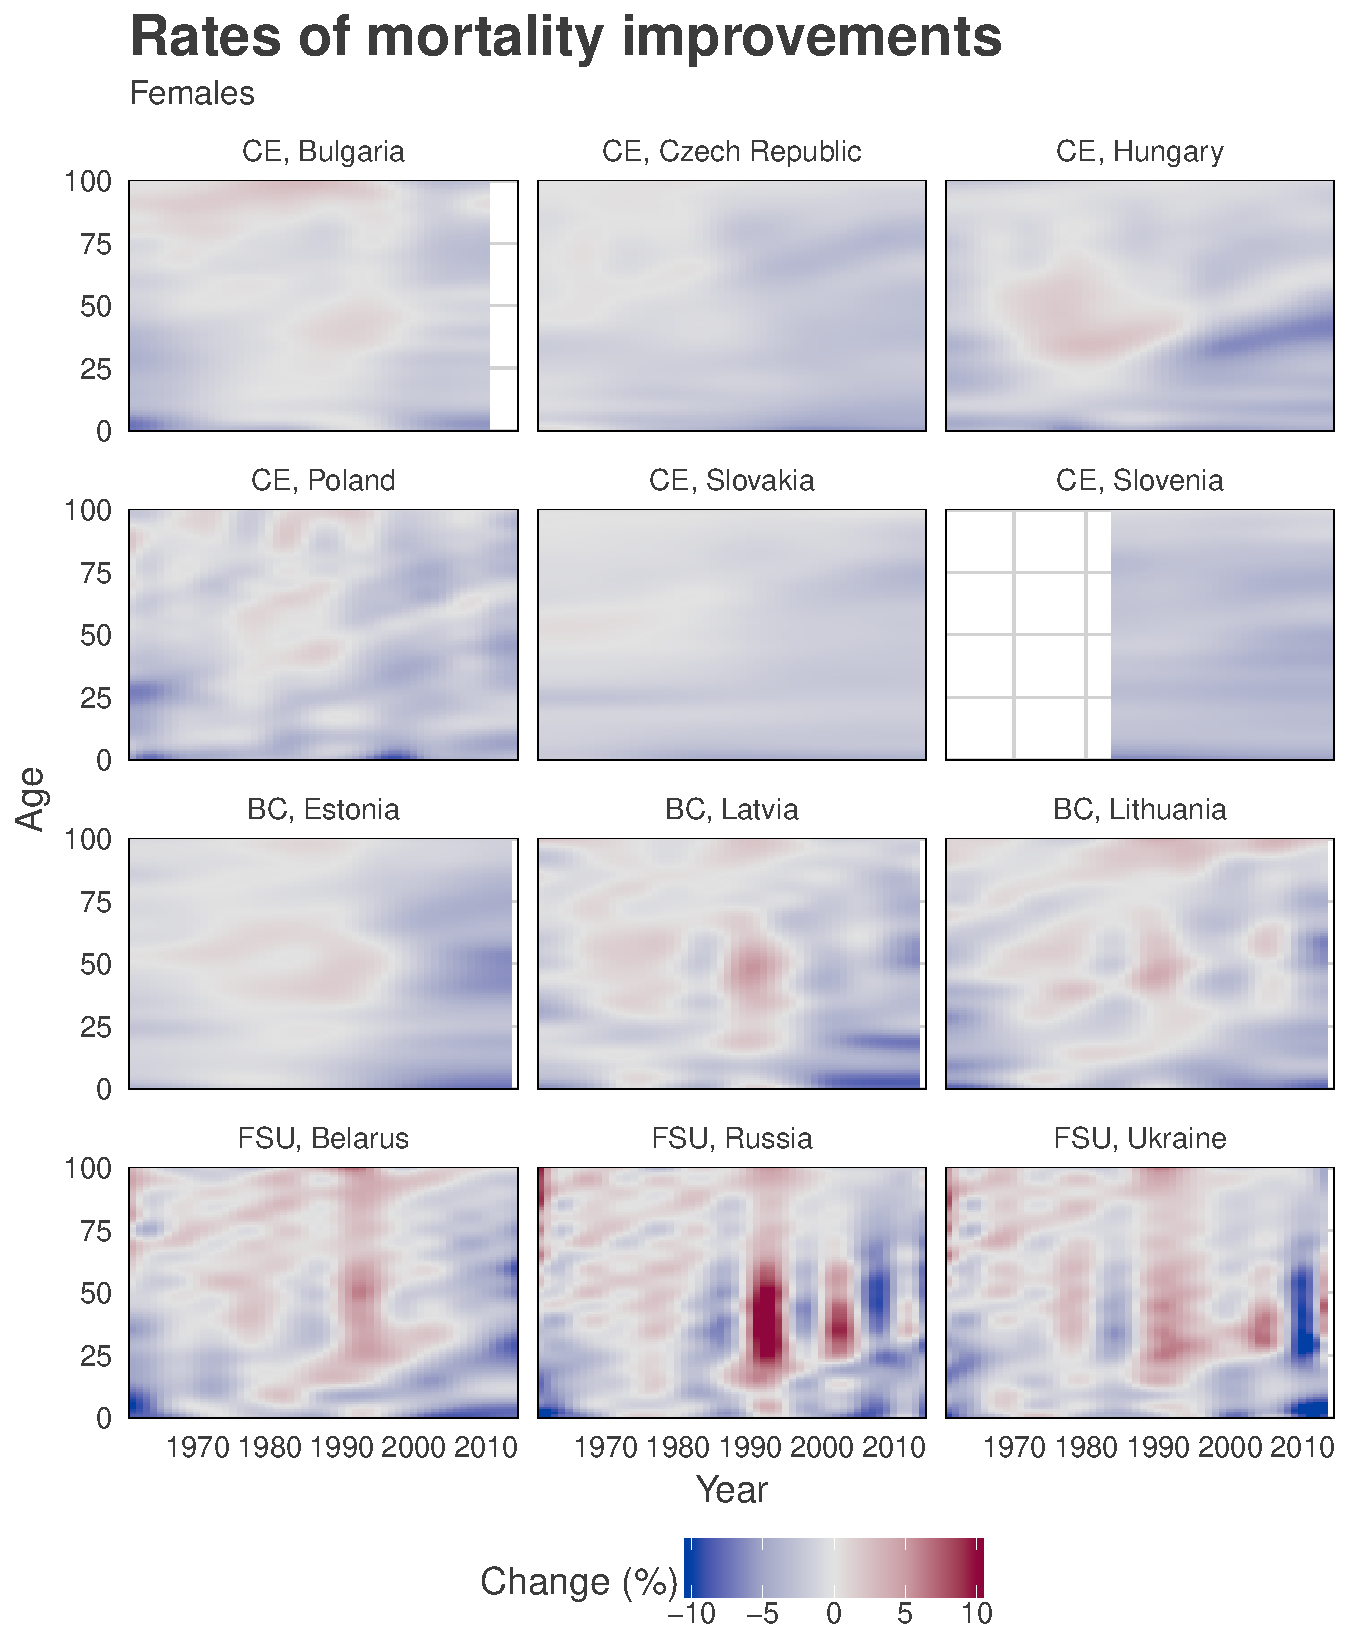
\includegraphics[scale=.55]{Figures/Romi_females.pdf}
\end{center}
Source: own calculations based on \citet{HMD} data. 
\begin{small}
Note: White areas indicate no data available
\end{small}
\end{figure}

\newpage

\begin{figure}[h!]
\centering
\caption{Trends in female life expectancy ($e_0$) and lifespan disparity  ($e^{\dagger}$) for 12 Eastern European countries, 1960-2014}
\begin{center}
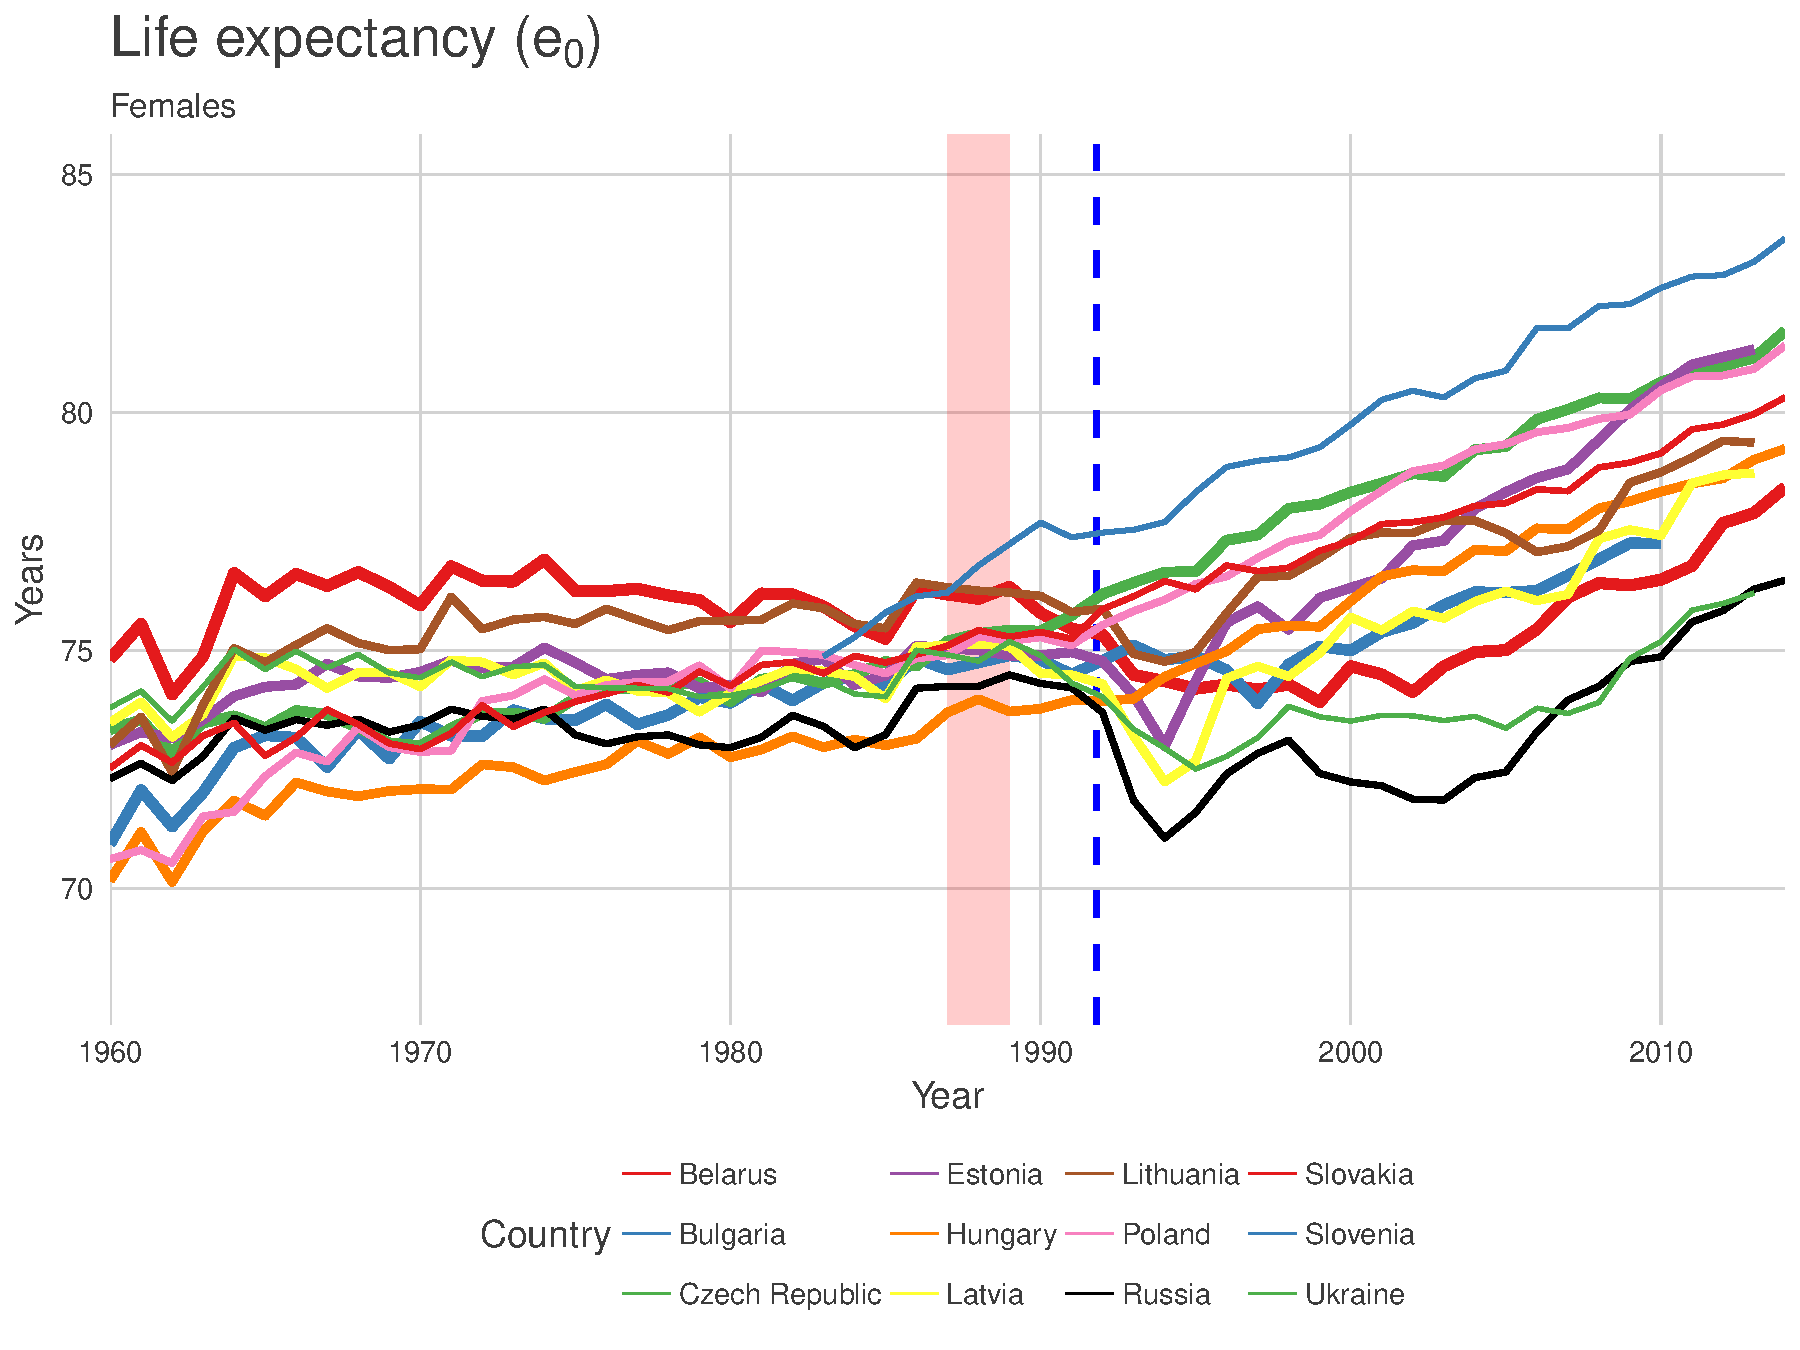
\includegraphics[scale=.40]{Figures/ex_females_labels.pdf}
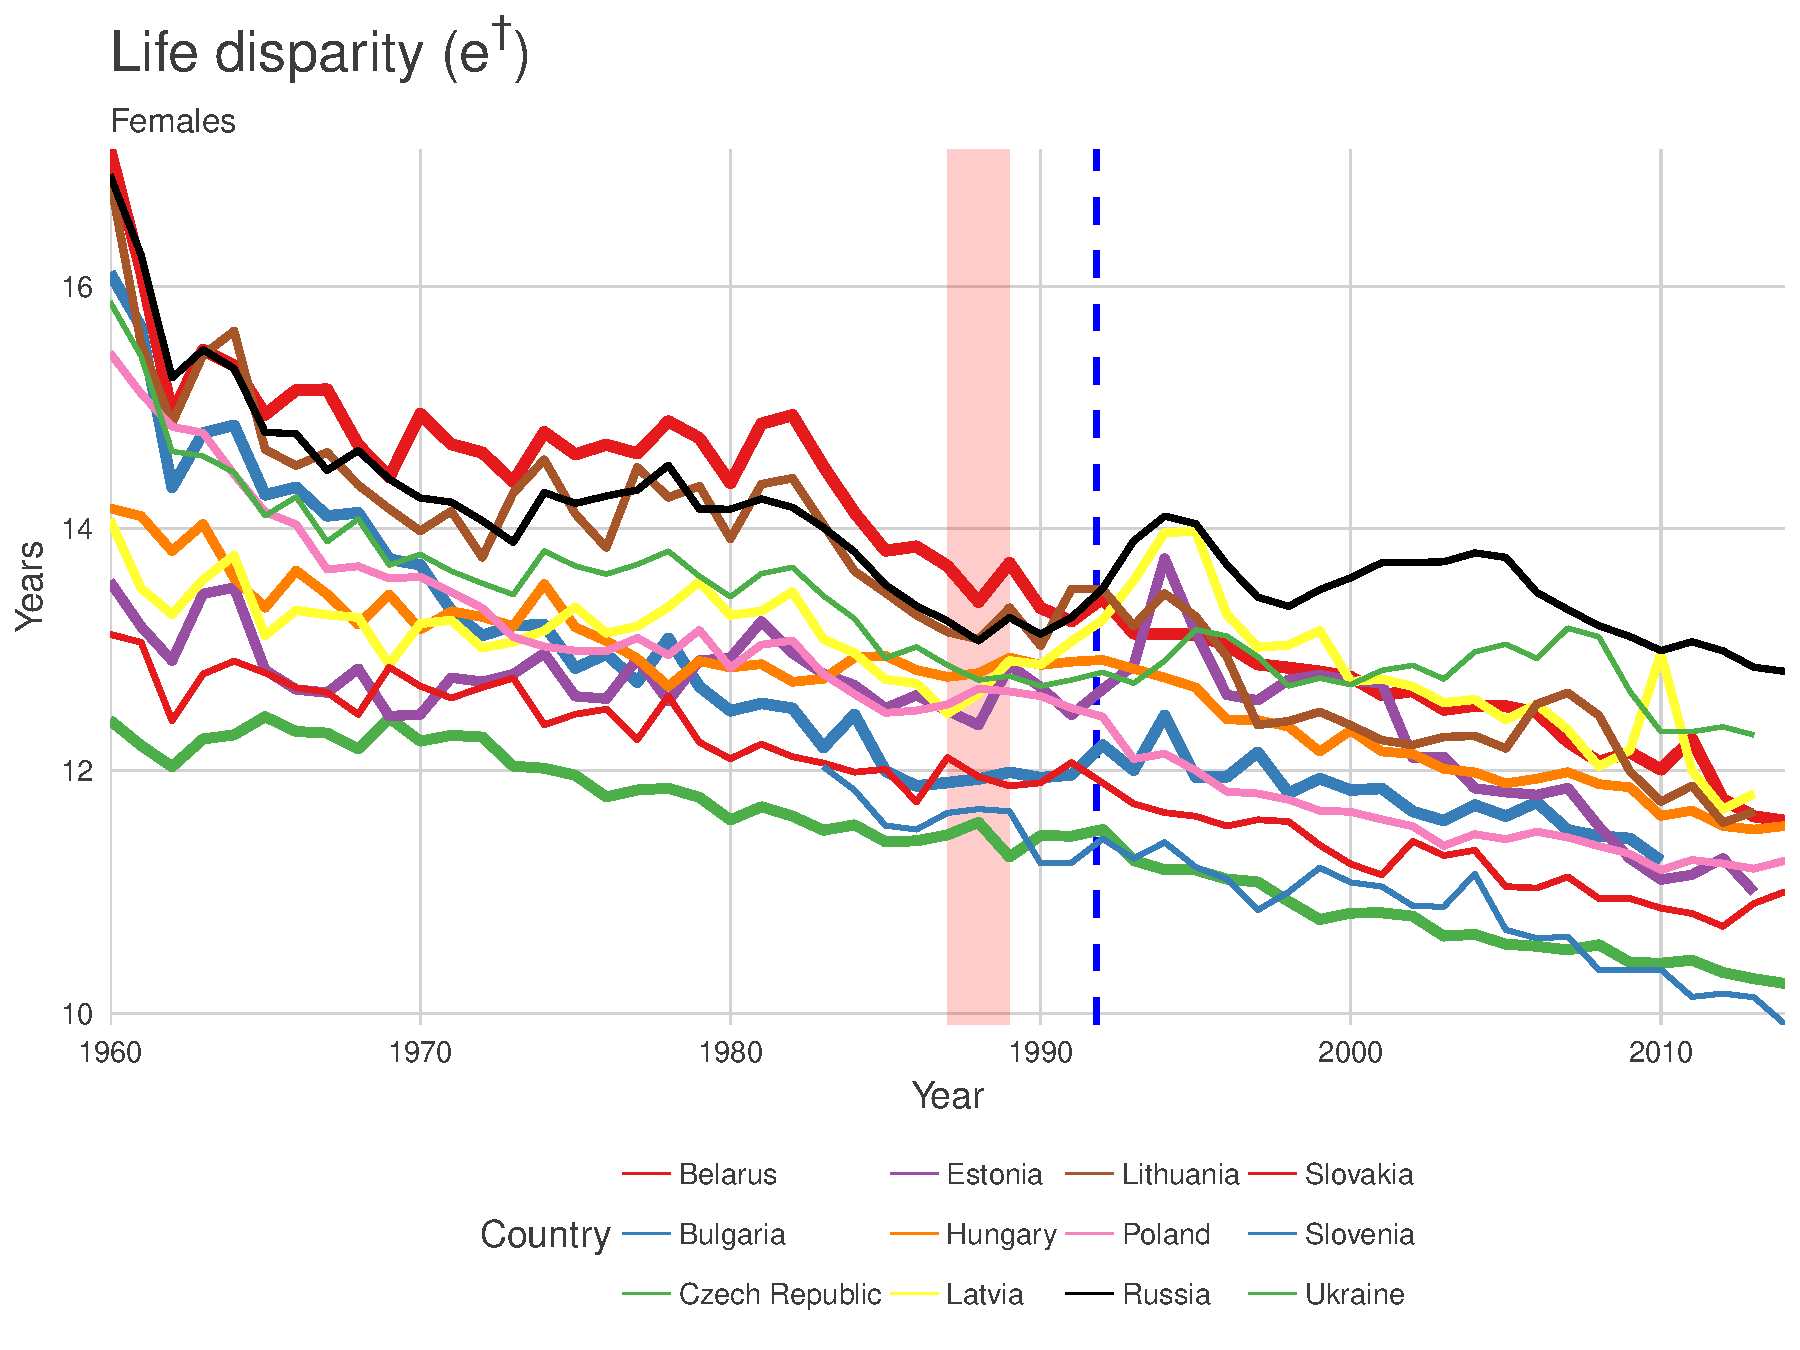
\includegraphics[scale=.40]{Figures/ed_females_labels.pdf}
\end{center}
Source: own calculations based on \citet{HMD} data. 
\end{figure}

\newpage

\begin{figure}[h!]
\centering
\caption{Absolute and relative yearly changes in life expectancy and lifespan disparity for females, 1960-2010}
\begin{center}
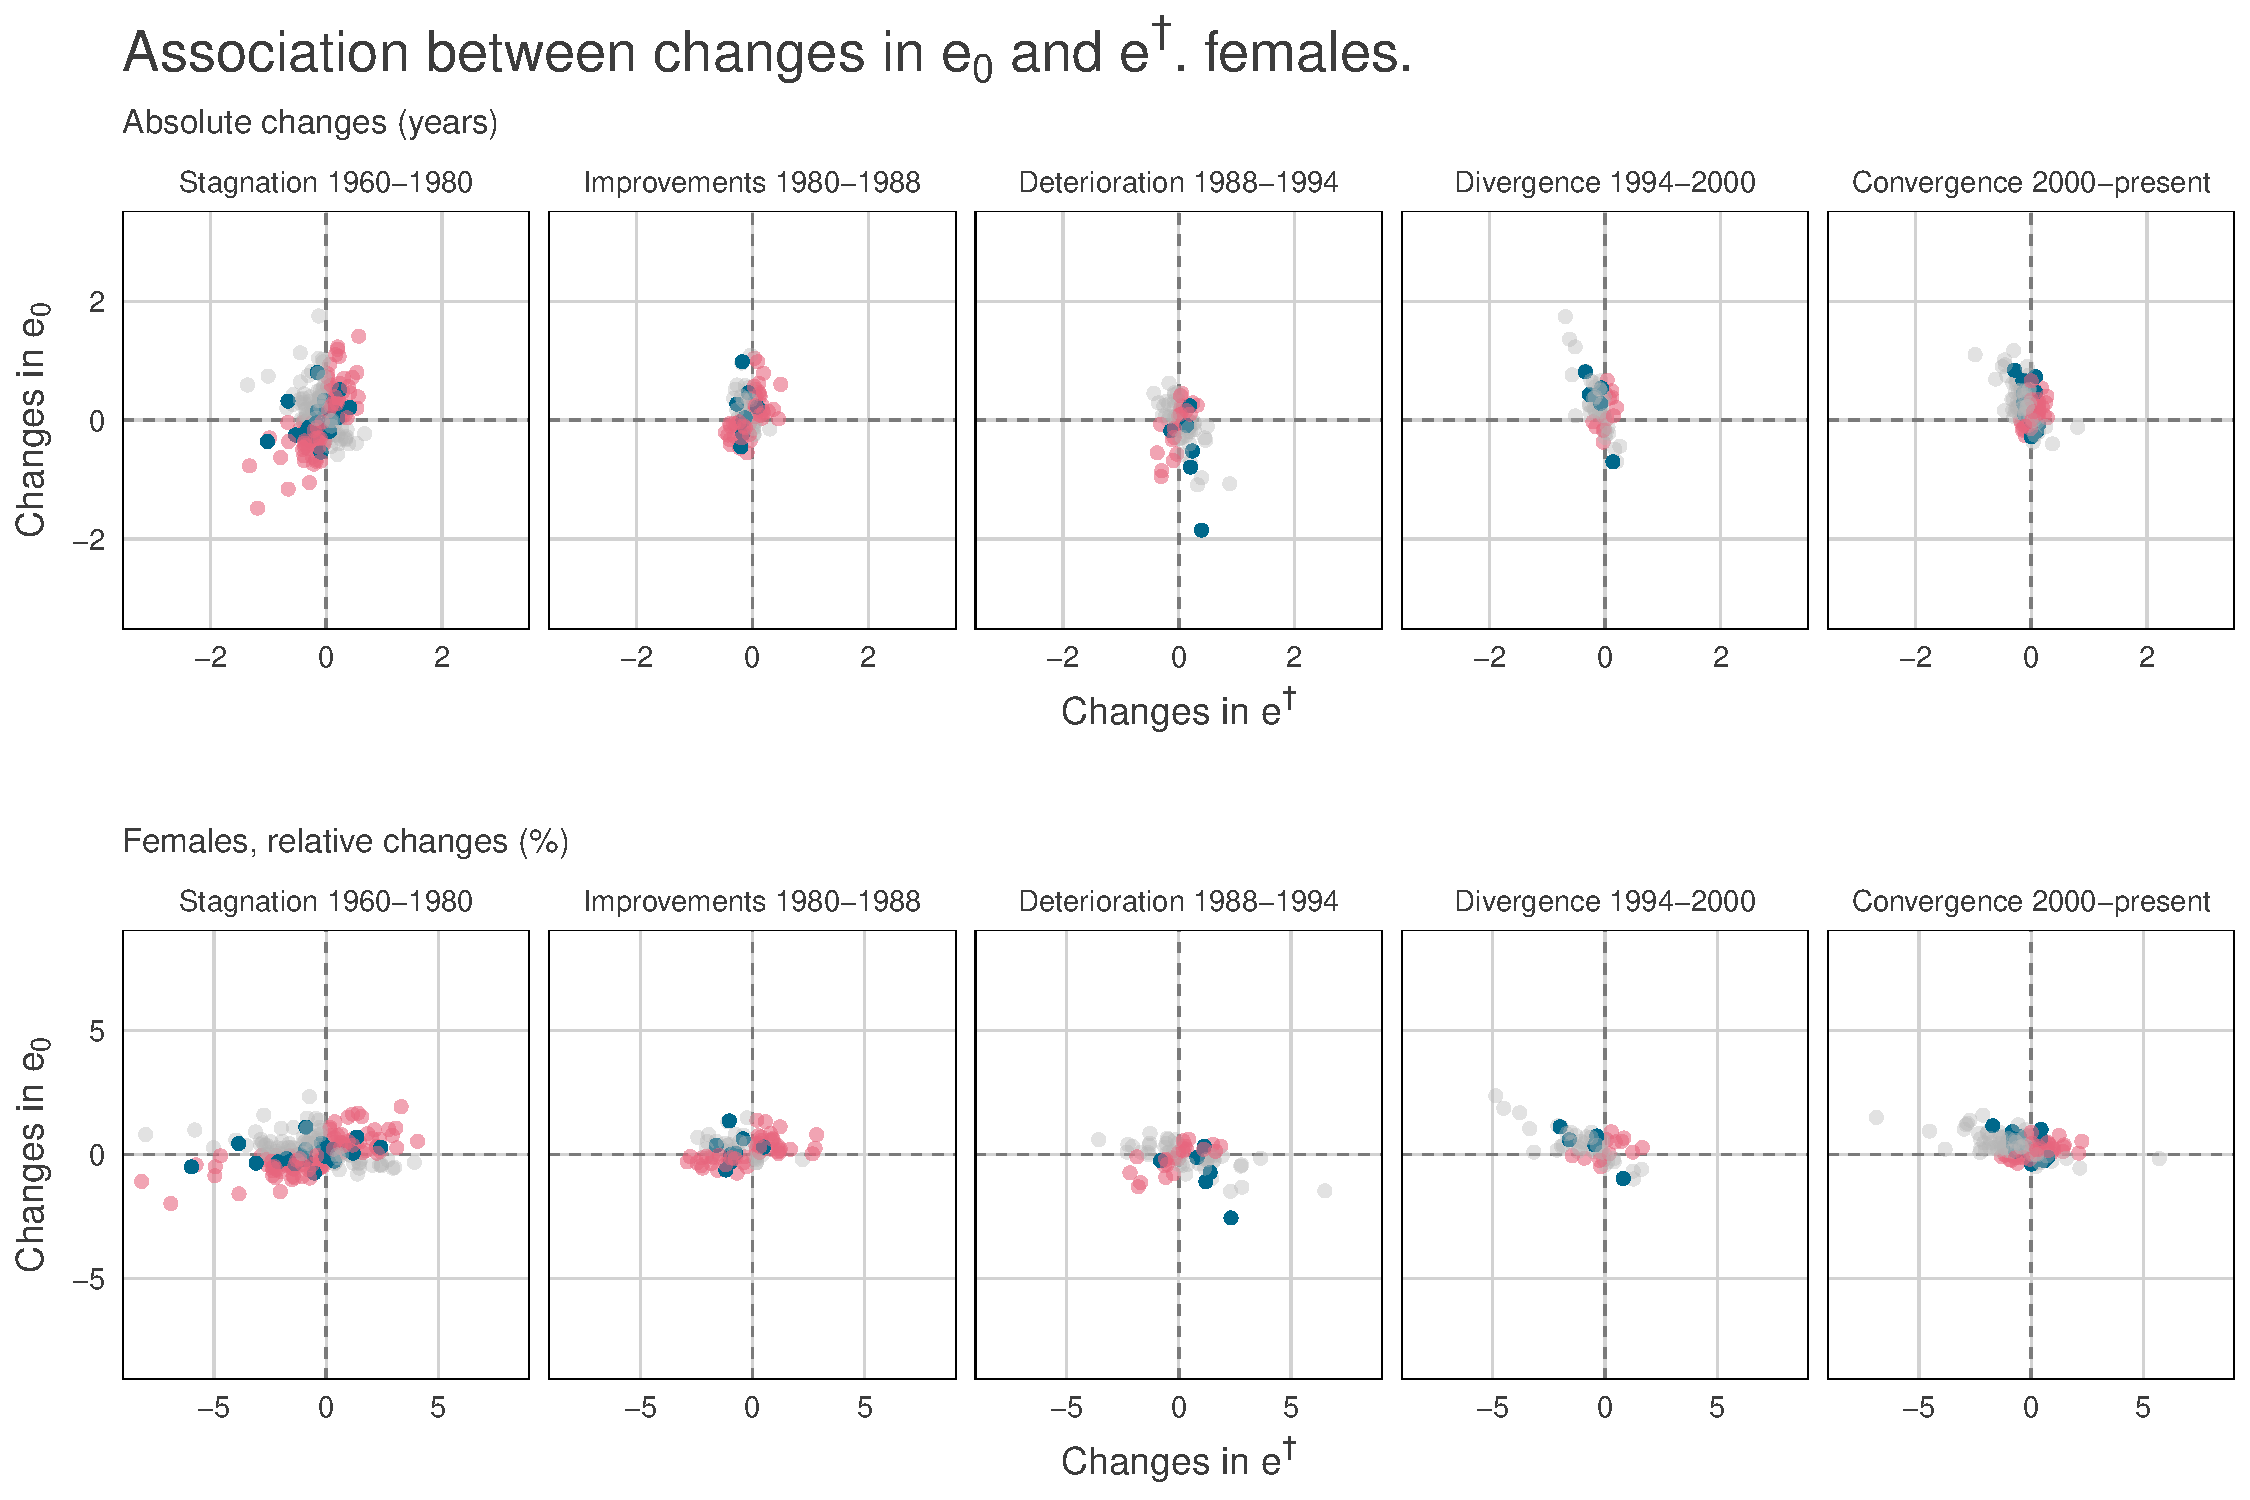
\includegraphics[scale=.47]{Figures/changes_females.pdf}
\end{center}
Source: own calculations based on \citet{HMD} data. Note: data for Slovenia begins in 1983. The dark dots are related to changes experienced in Russia.
\end{figure}

\newpage

\begin{figure}[h!]
\caption{Age-specific contributions to the change in lifespan disparity $e^\dagger$ by periods, females.}
\centering
\begin{center}
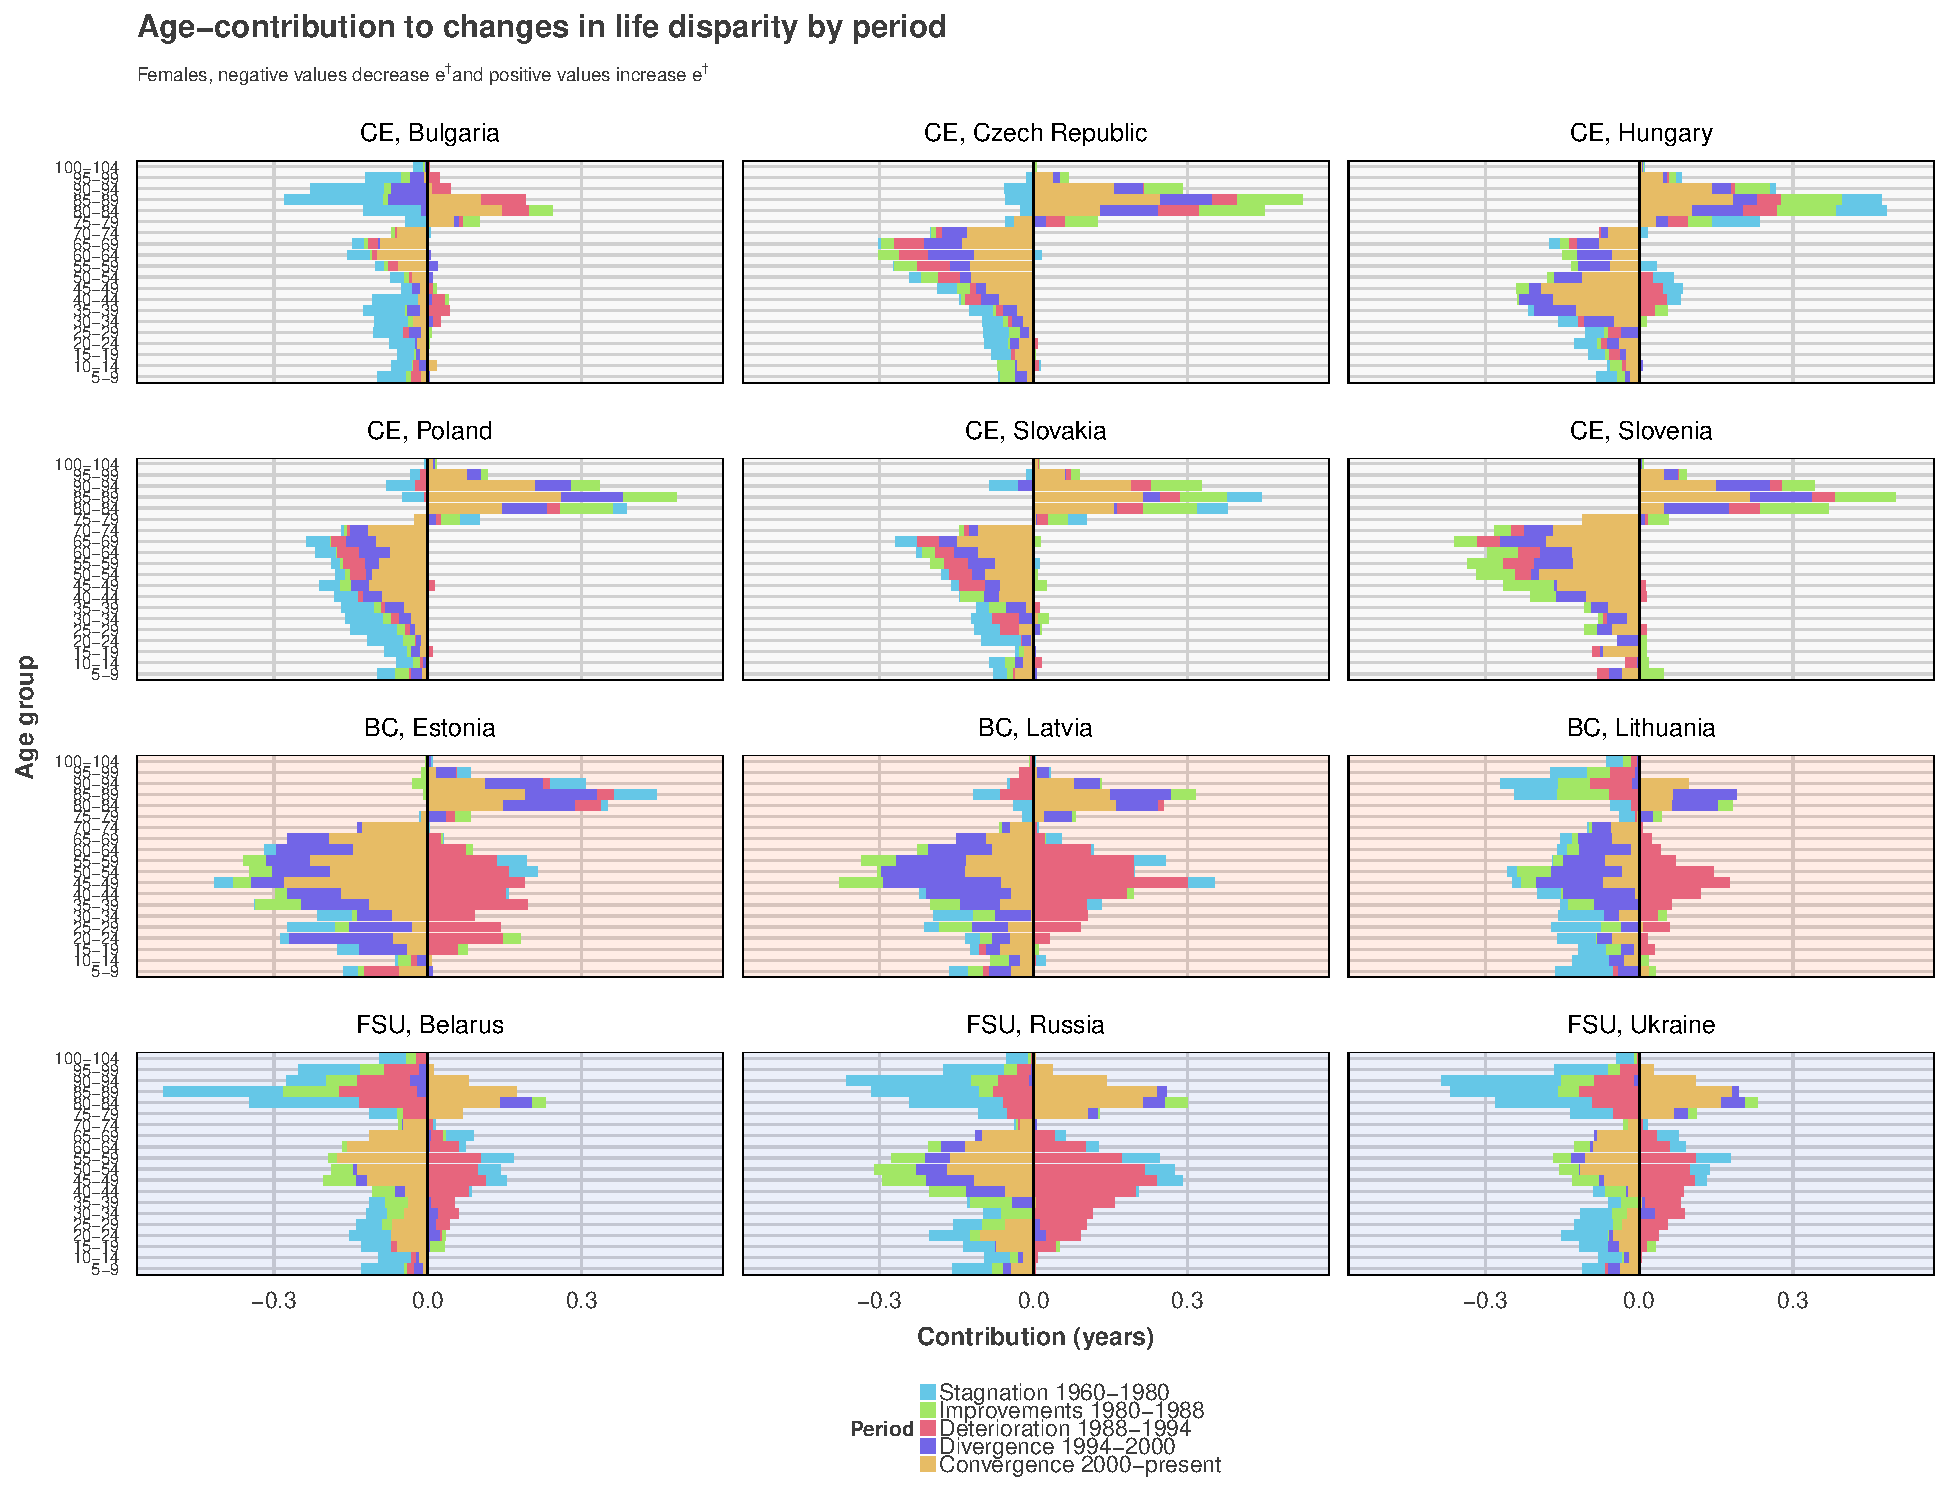
\includegraphics[scale=.46]{Figures/Age_ed_decomp_Females.pdf}
\end{center}
Source: own calculations based on \citet{HMD} data. Note: data for Slovenia begins in 1983.
\end{figure}

\newpage

\begin{figure}[h!]
\caption{Cause specific contributions to the change in  female lifespan disparity  $e^\dagger$, 1994-2000}
\centering
\begin{center}
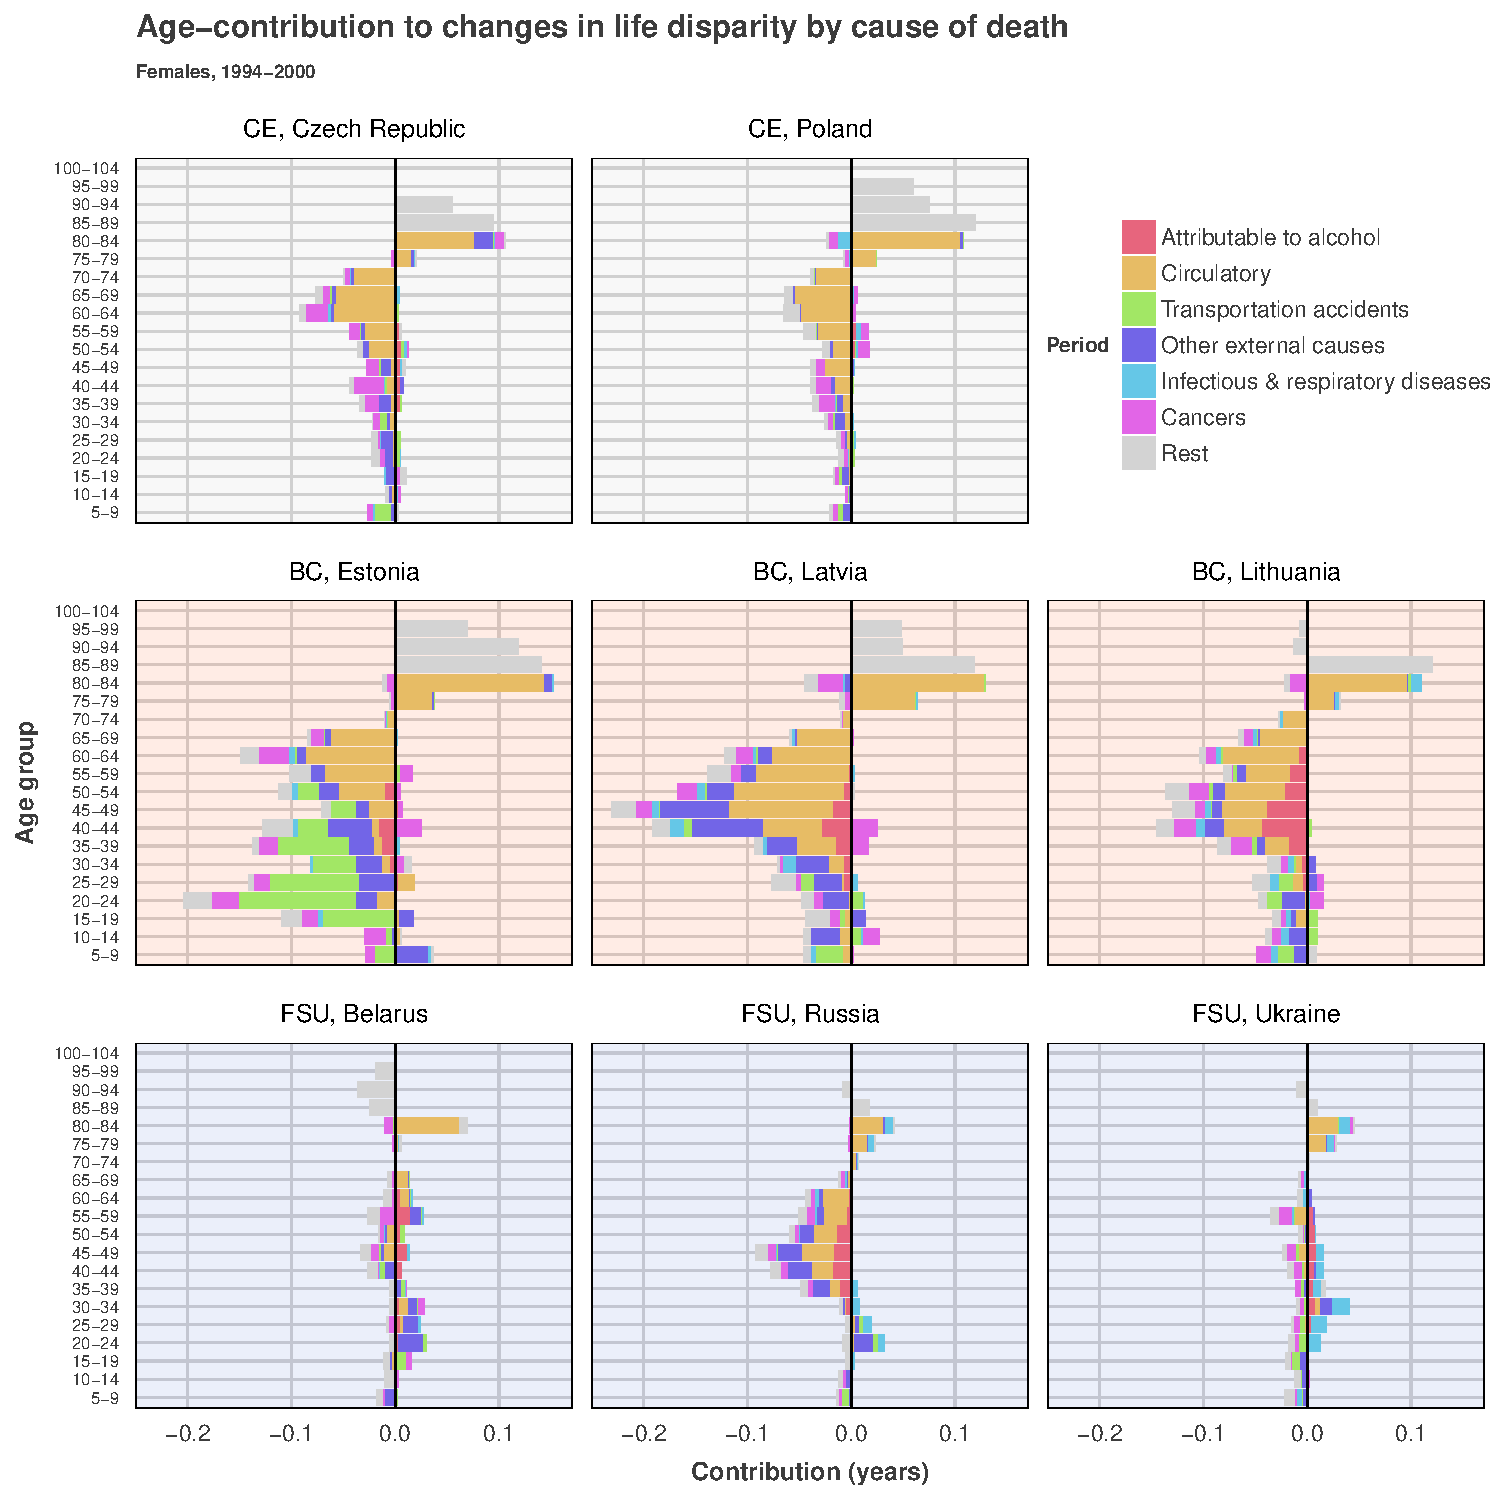
\includegraphics[scale=.5]{Figures/Cause_ed_decomp_Females_1.pdf}
\end{center}
Source: own calculations based on \citet{HMD} data. 
\end{figure}

\newpage

\begin{figure}[h!]
\caption{Cause specific contributions to the change in  female lifespan disparity  $e^\dagger$, 2000-2010}
\centering
\begin{center}
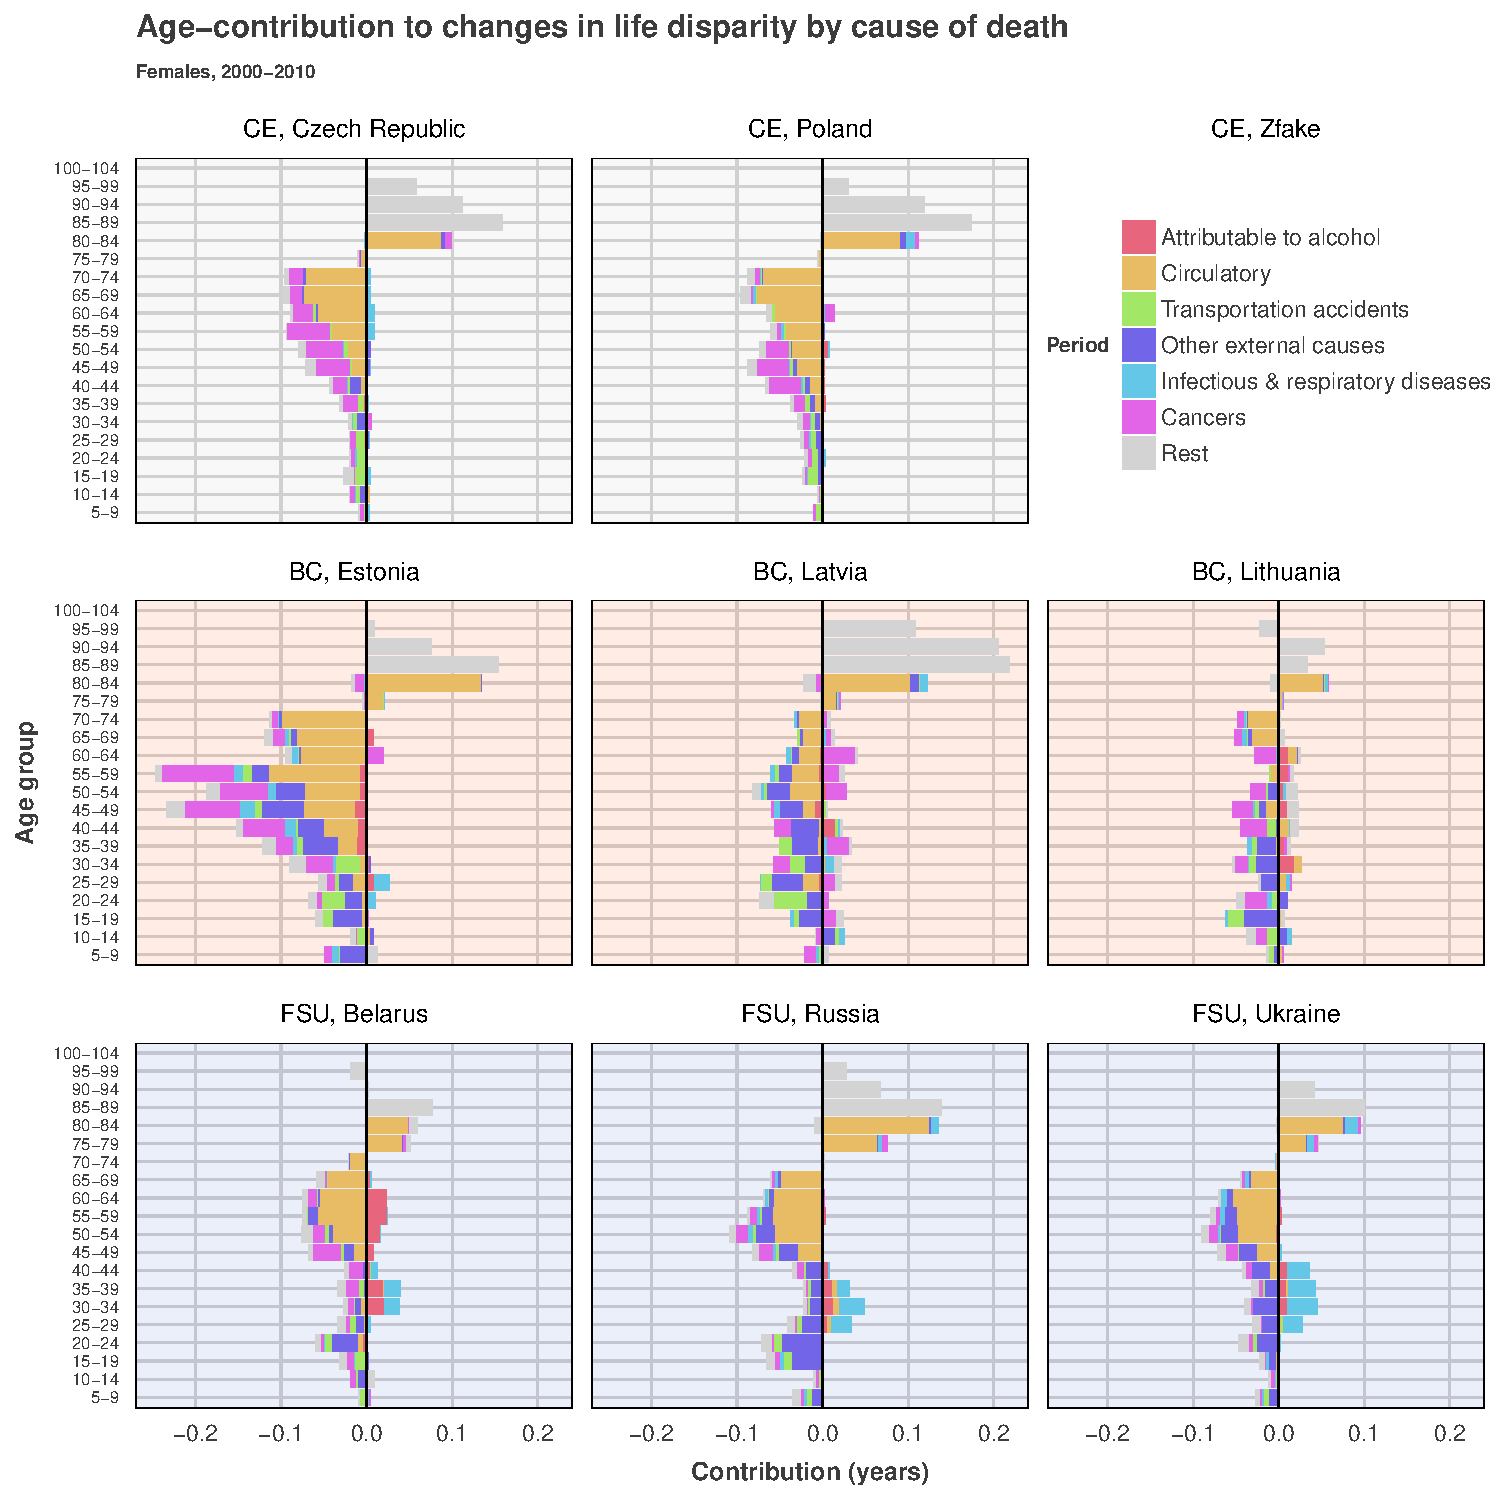
\includegraphics[scale=.5]{Figures/Cause_ed_decomp_Females_2.pdf}
\end{center}
Source: own calculations based on \citet{HMD} data. Note: data for Poland ends in 2009.
\end{figure}

\newpage



\section*{Infant contributions to changes in $e^\dagger$ and $e_0$}

\begin{figure}[h!]
\centering
\caption{Infant contributions, below age 5, to changes in $e^\dagger$ and $e_0$ by period and sex}
\label{Fig_LE&LD}
\begin{center}
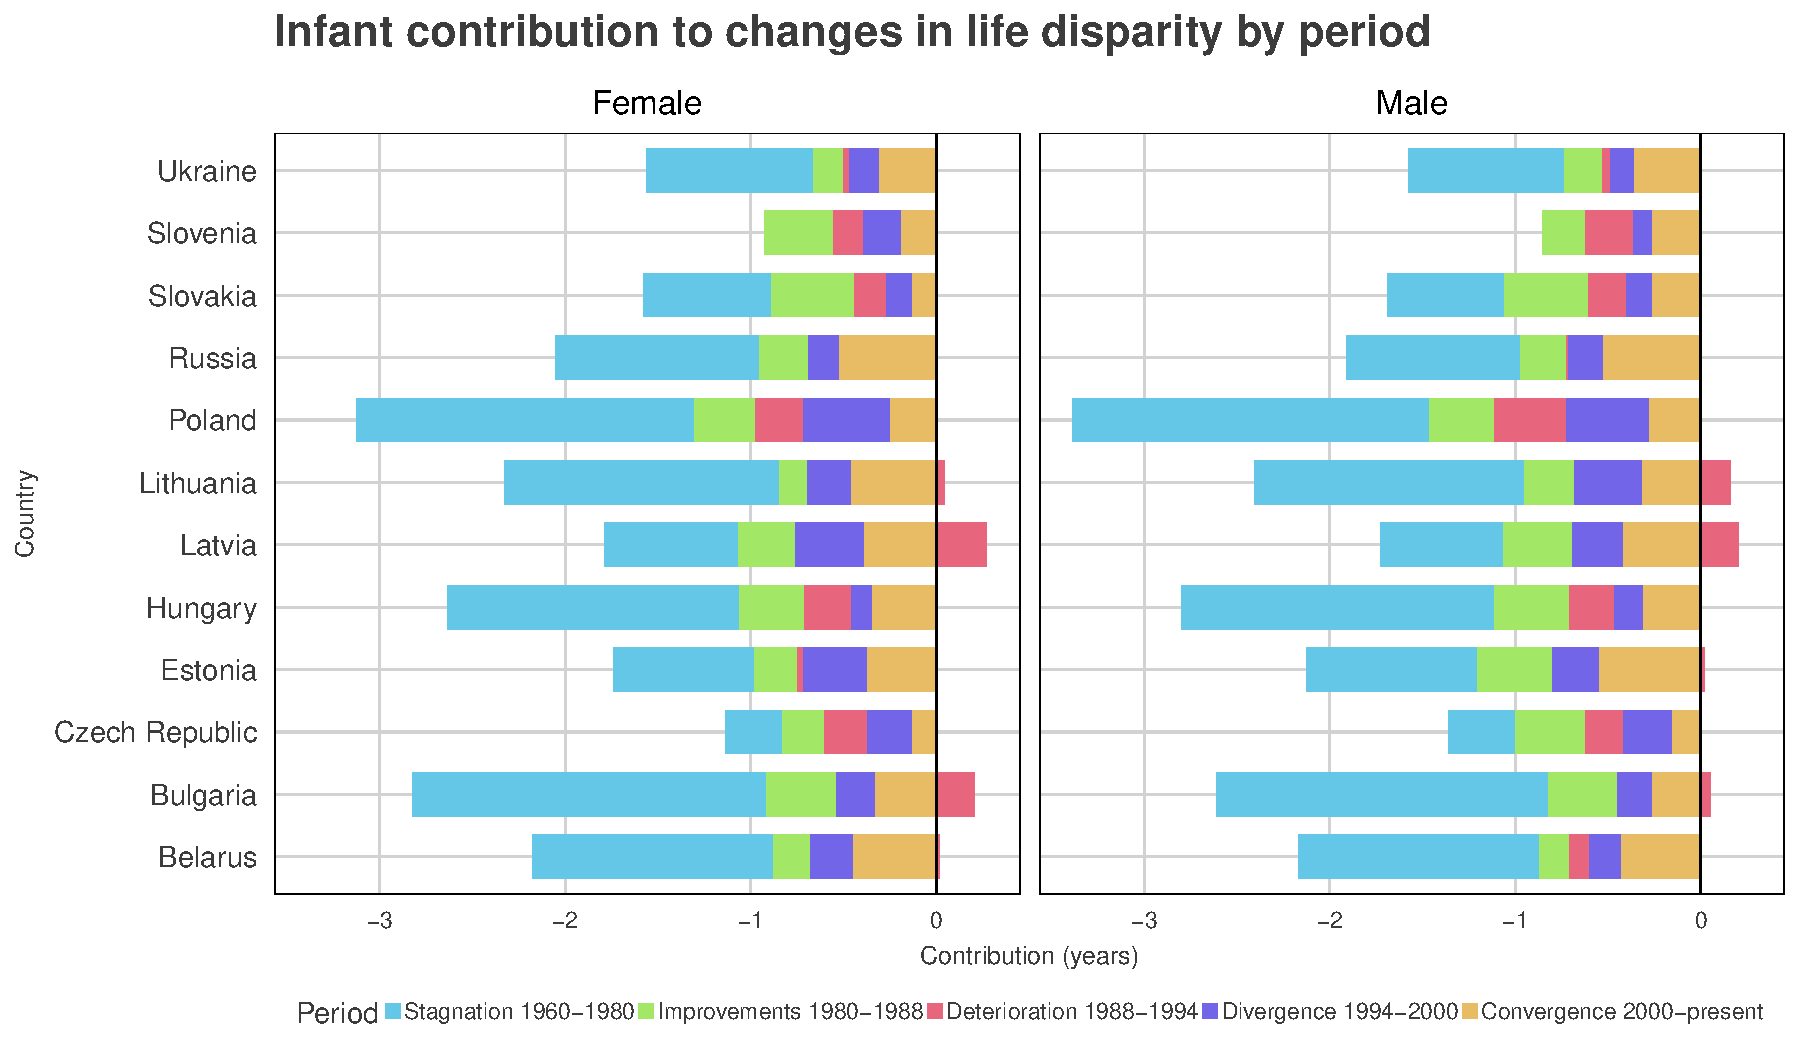
\includegraphics[scale=.5]{Figures/Infant_ed_decomp.pdf}
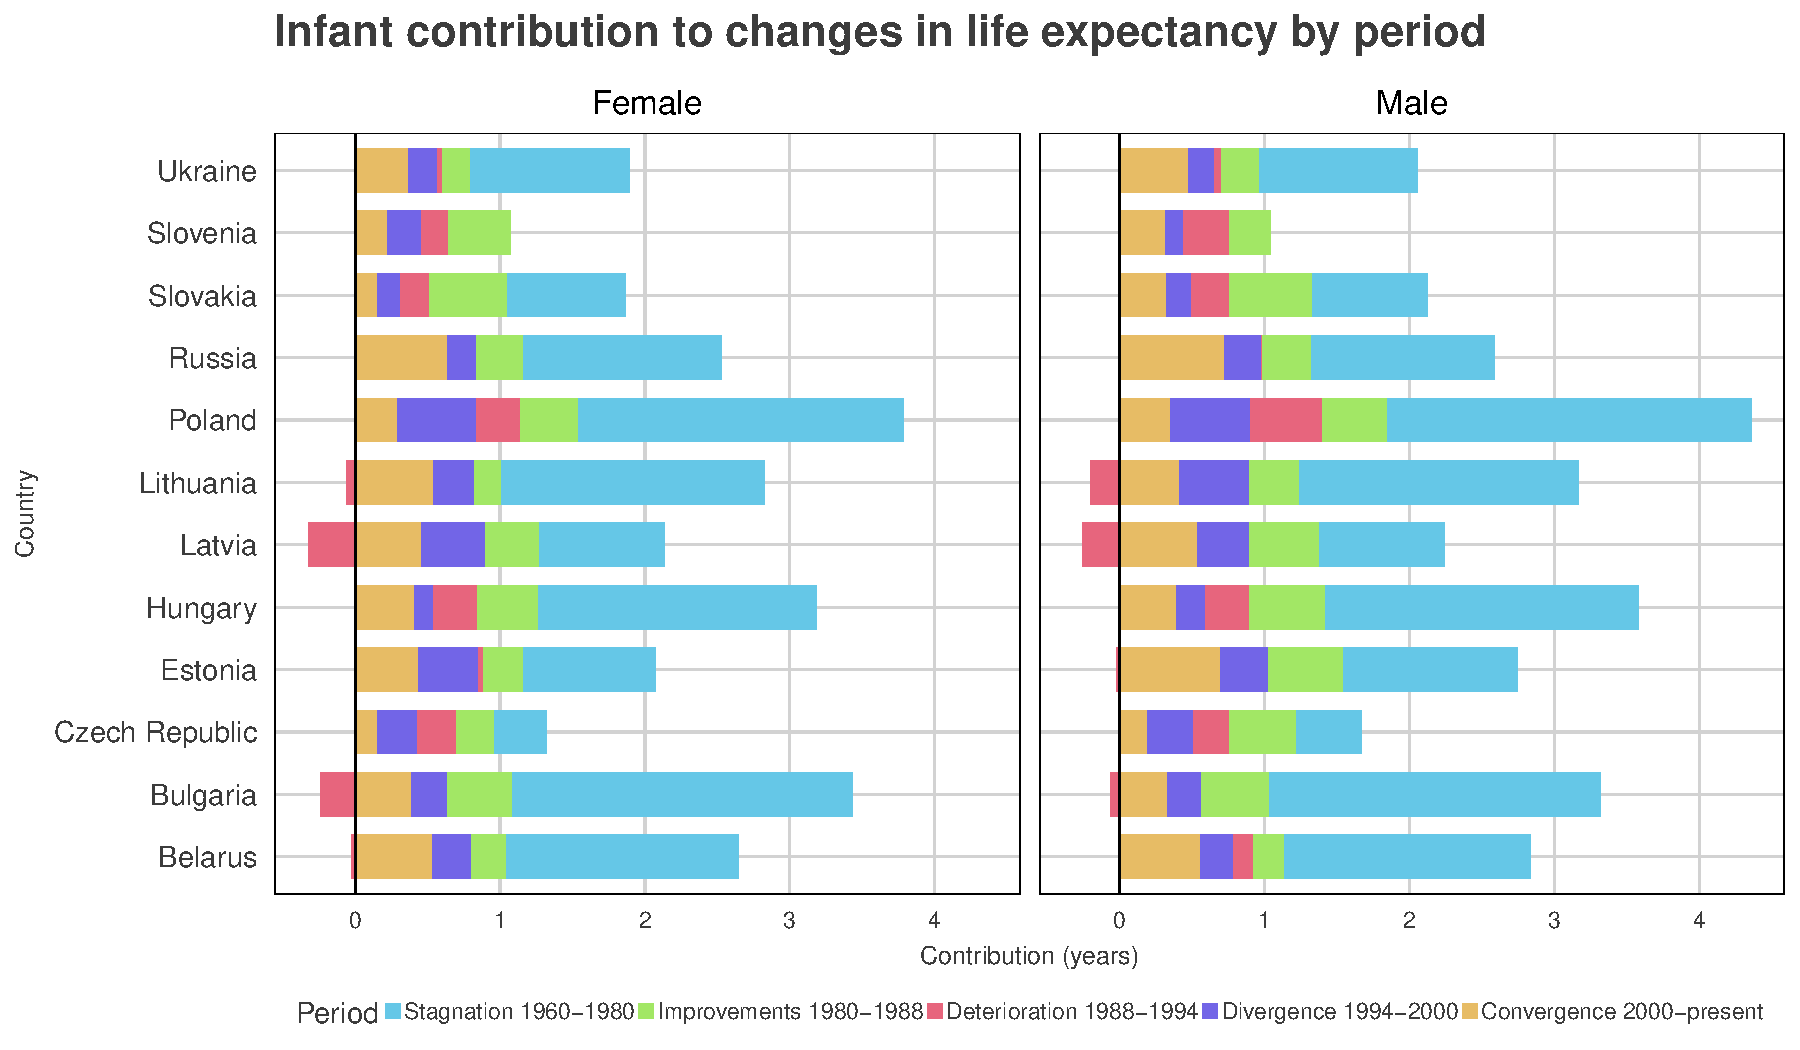
\includegraphics[scale=.5]{Figures/Infant_ex_decomp.pdf}
\end{center}
Source: own calculations based on \citet{HMD} data. 
\end{figure}

\newpage

\section*{Age and age-cause specific decomposition results for life expectancy}


\begin{figure}[h!]
\caption{Age-specific contributions to the change in $e_0$ by periods for males.}
\centering
\begin{center}
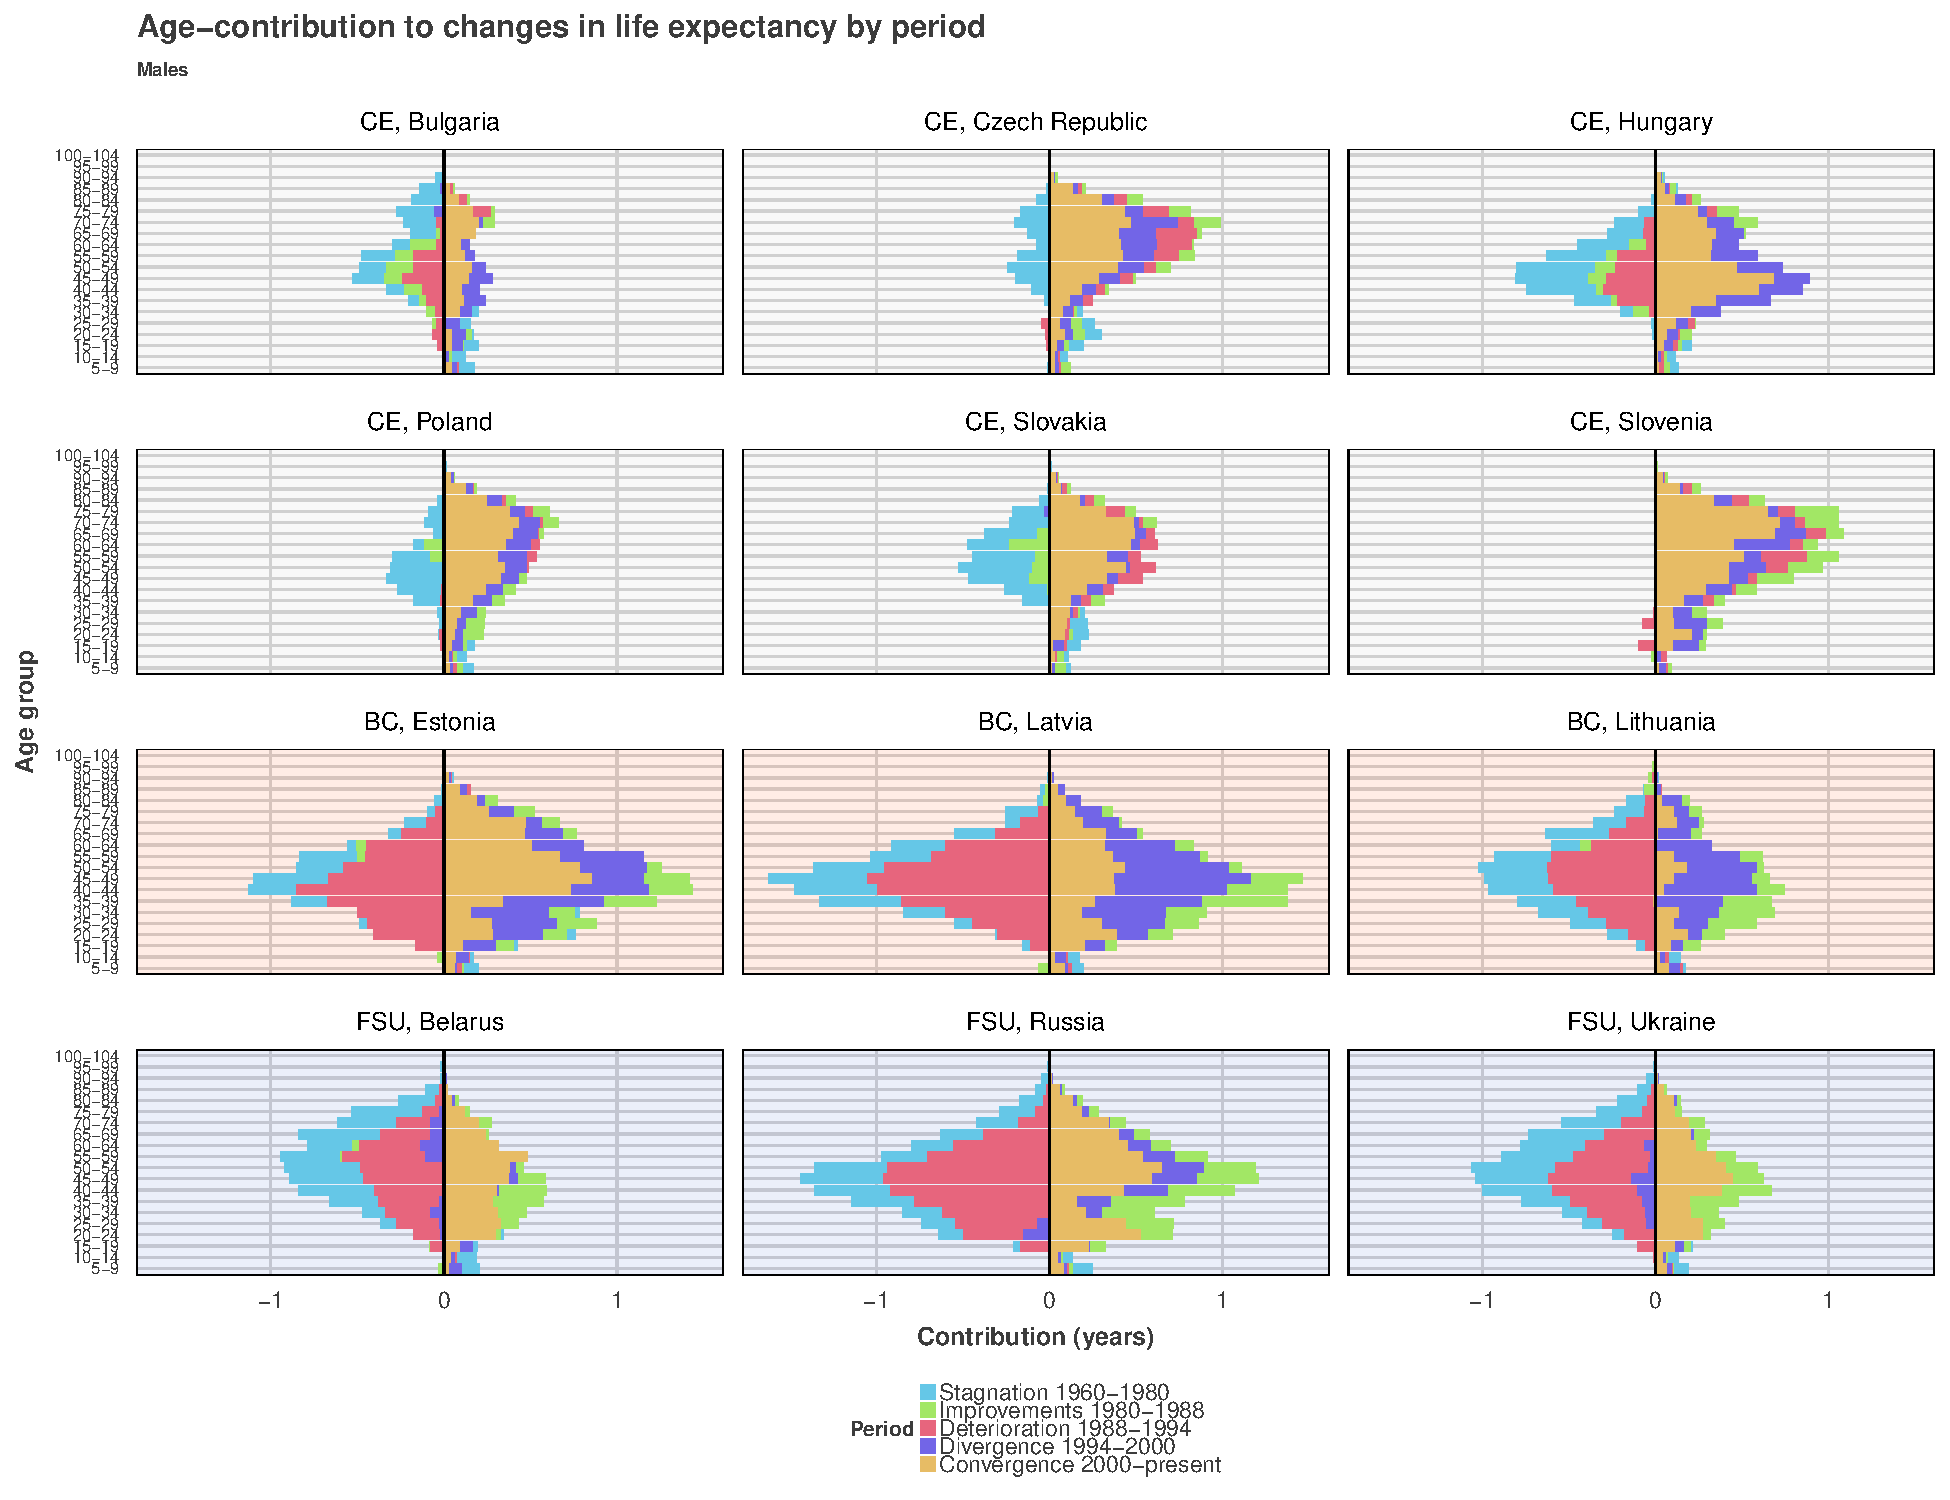
\includegraphics[scale=.46]{Figures/Age_e0_decomp_Males.pdf}
\end{center}
Source: own calculations based on \citet{HMD} data. Note: data for Slovenia begins in 1983.
\end{figure}

\newpage

\begin{figure}[h!]
\caption{Age-specific contributions to the change in $e_0$ by periods for females.}
\centering
\begin{center}
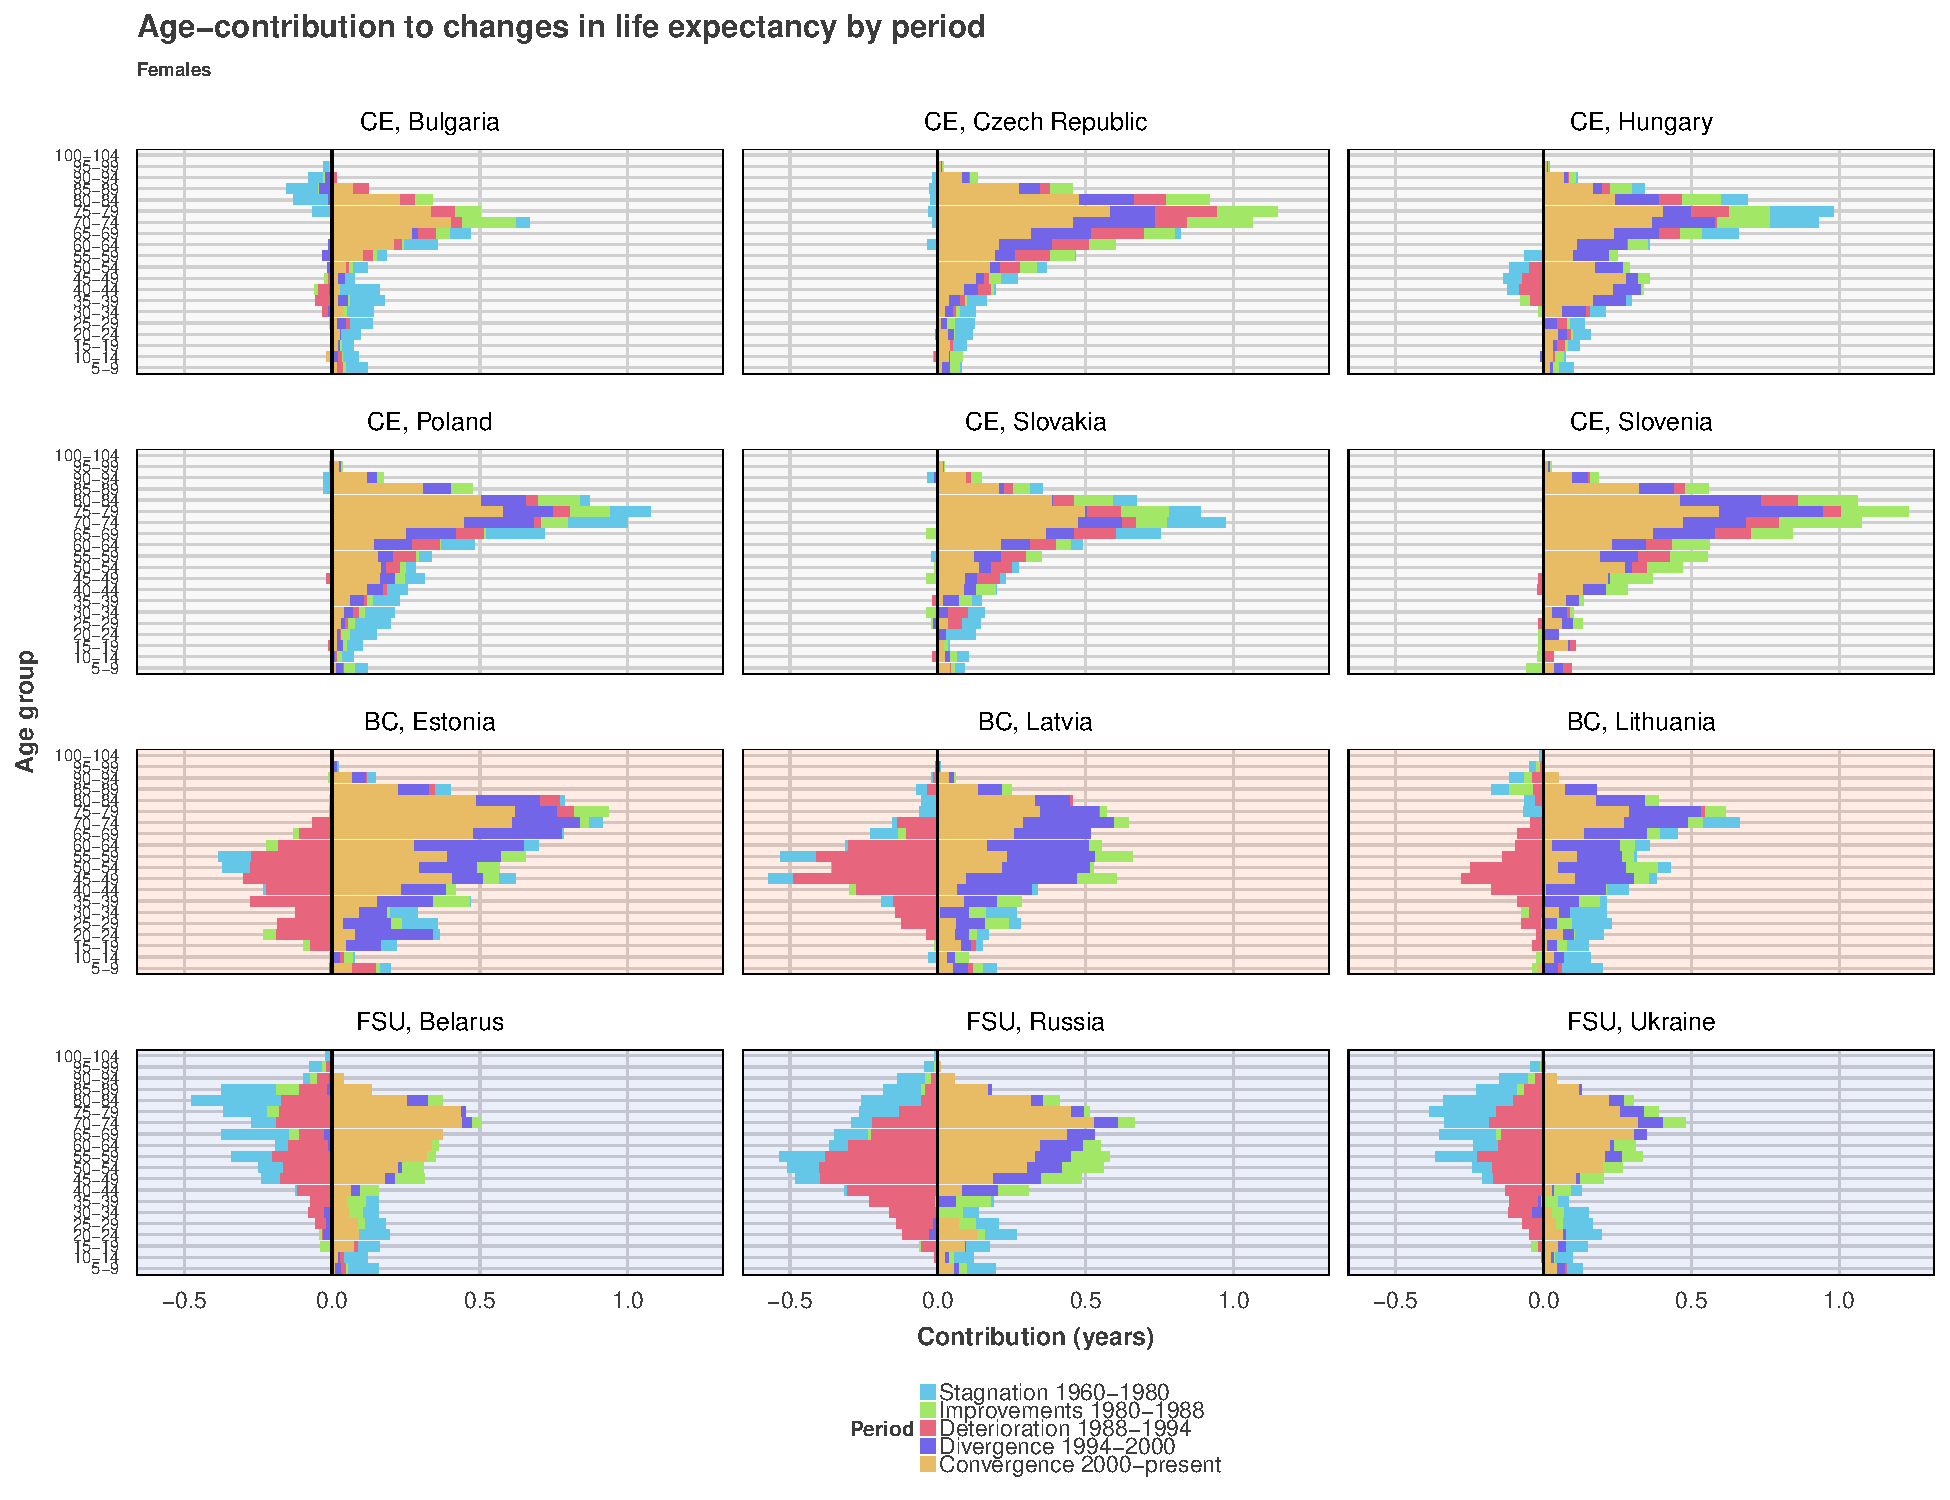
\includegraphics[scale=.46]{Figures/Age_e0_decomp_Females.pdf}
\end{center}
Source: own calculations based on \citet{HMD} data. Note: data for Slovenia begins in 1983.
\end{figure}

\newpage

\begin{figure}[h!]
\caption{Age-cause-specific contributions to the change in $e_0$ by periods for males 1994-2000.}
\centering
\begin{center}
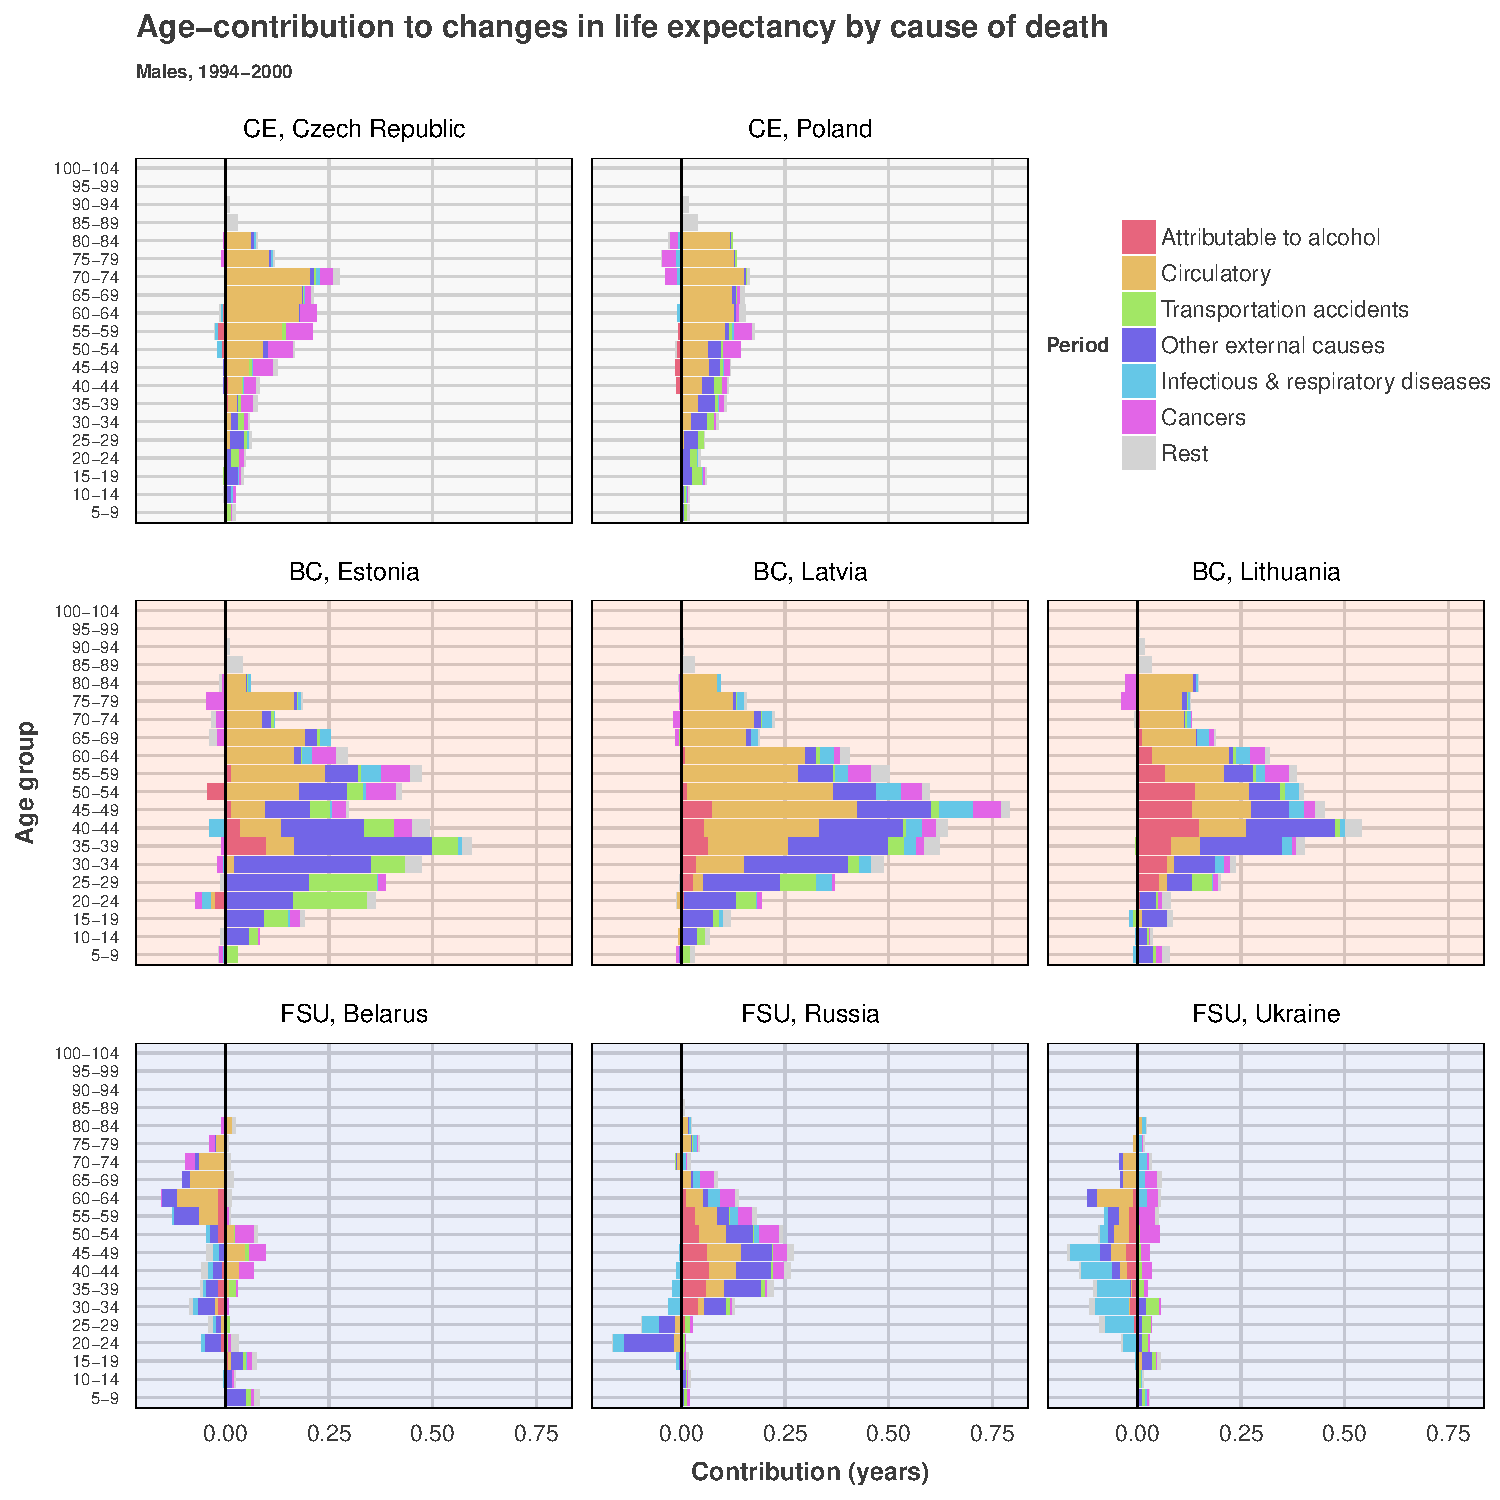
\includegraphics[scale=.5]{Figures/Cause_e0_decomp_Males_1.pdf}
\end{center}
Source: own calculations based on \citet{HMD} data. Note: data for Slovenia begins in 1983.
\end{figure}

\newpage
\begin{figure}[h!]
\caption{Age-cause-specific contributions to the change in $e_0$ by periods for males 2000-2010.}
\centering
\begin{center}
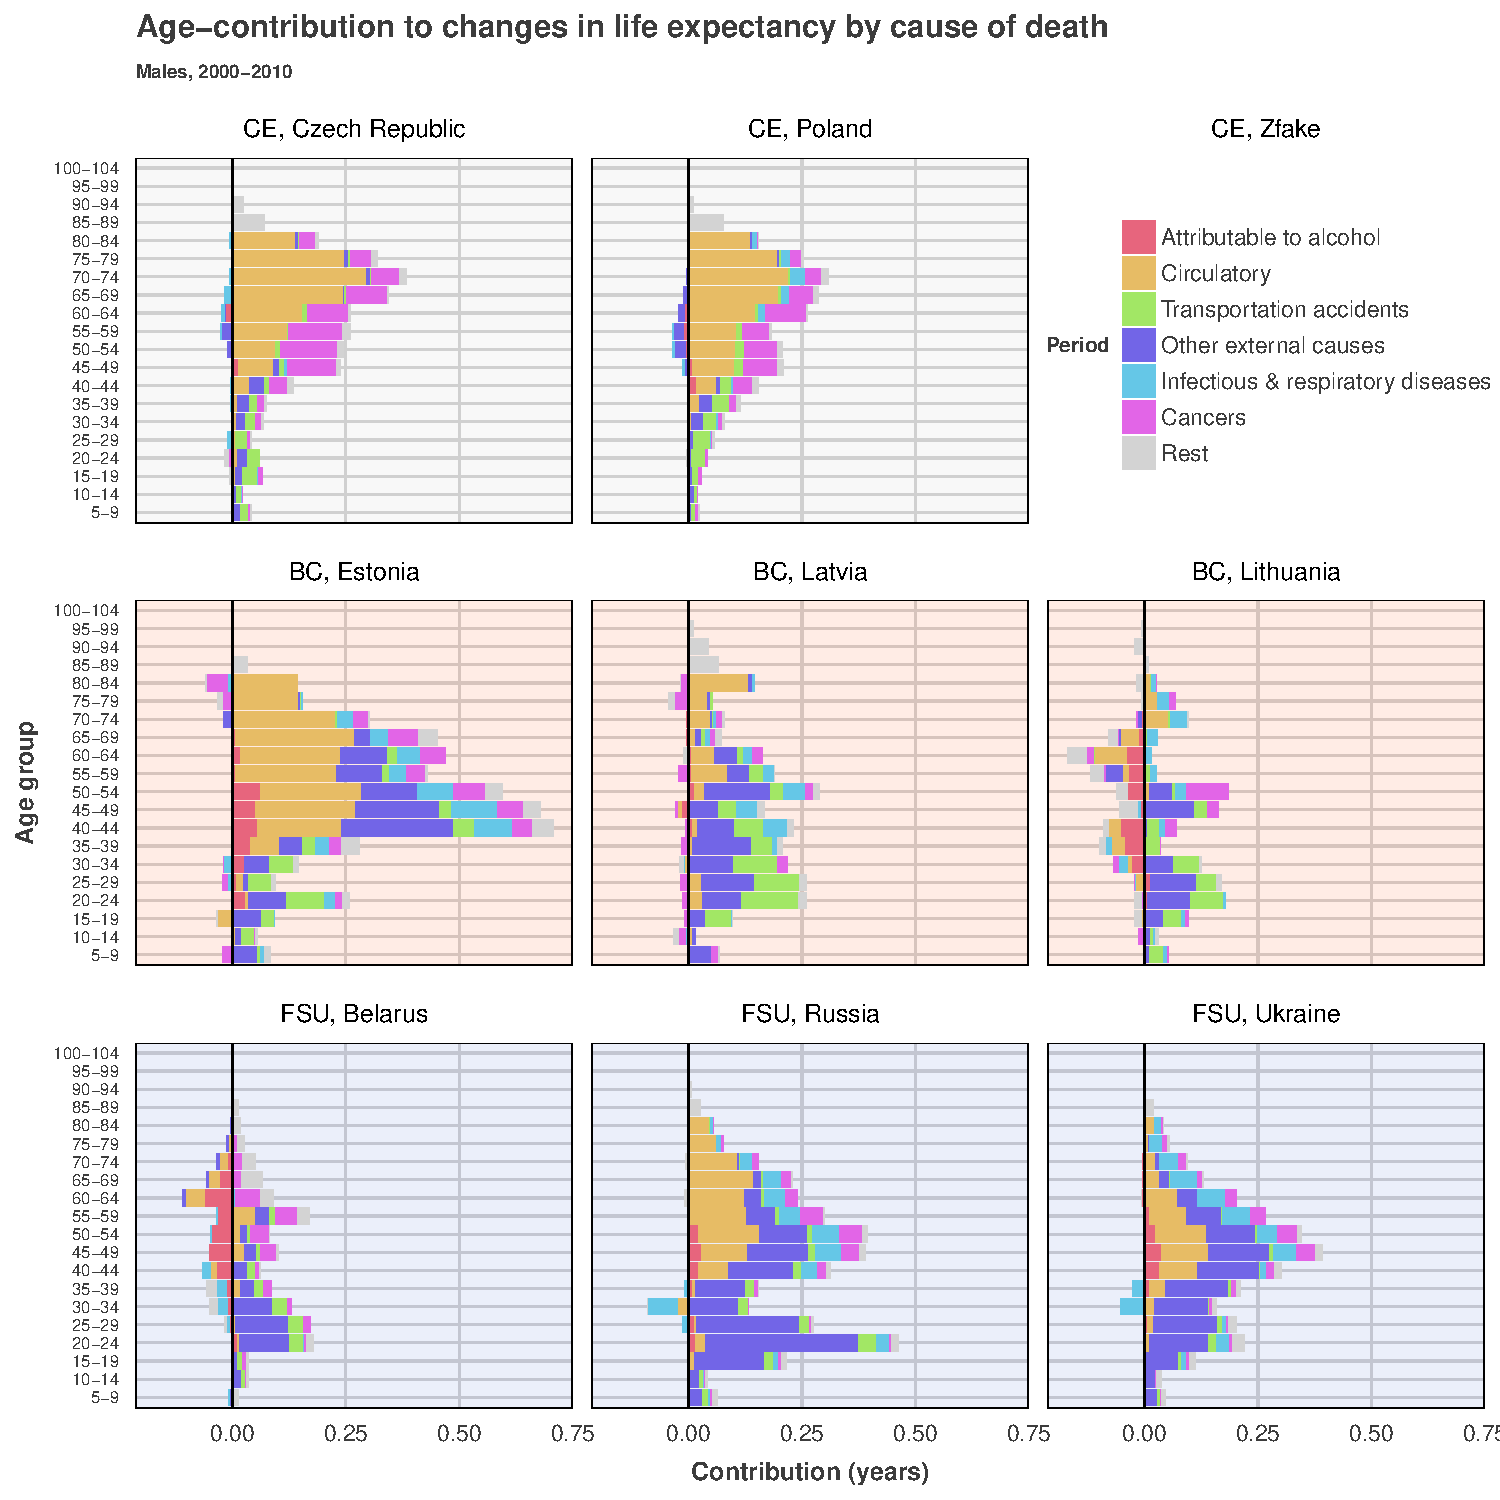
\includegraphics[scale=.5]{Figures/Cause_e0_decomp_Males_2.pdf}
\end{center}
Source: own calculations based on \citet{HMD} data. Note: data for Slovenia begins in 1983.
\end{figure}

\newpage

\begin{figure}[h!]
\caption{Age-cause-specific contributions to the change in $e_0$ by periods for females 1994-2000.}
\centering
\begin{center}
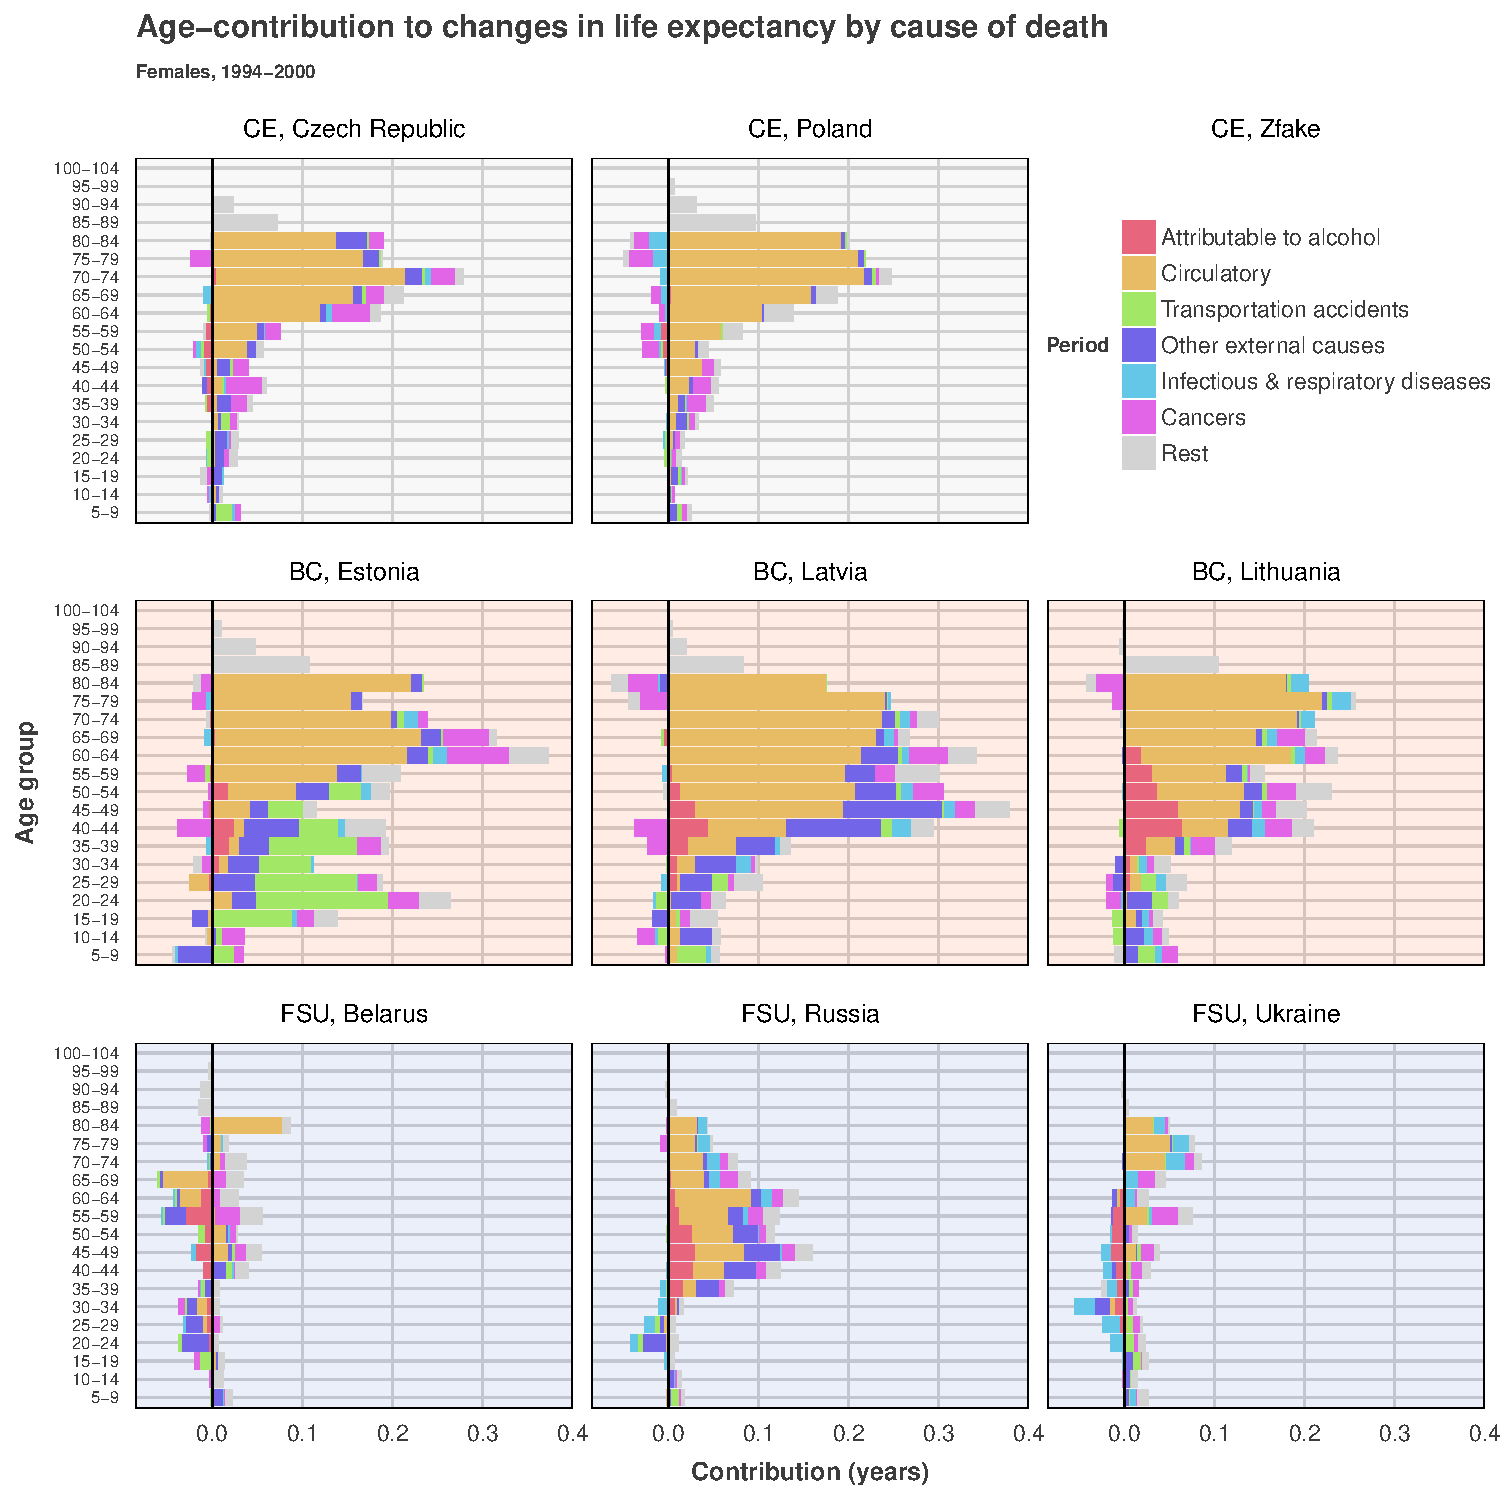
\includegraphics[scale=.5]{Figures/Cause_e0_decomp_Females_1.pdf}
\end{center}
Source: own calculations based on \citet{HMD} data. Note: data for Slovenia begins in 1983.
\end{figure}

\newpage

\begin{figure}[h!]
\caption{Age-cause-specific contributions to the change in $e_0$ by periods for females 2000-2010.}
\centering
\begin{center}
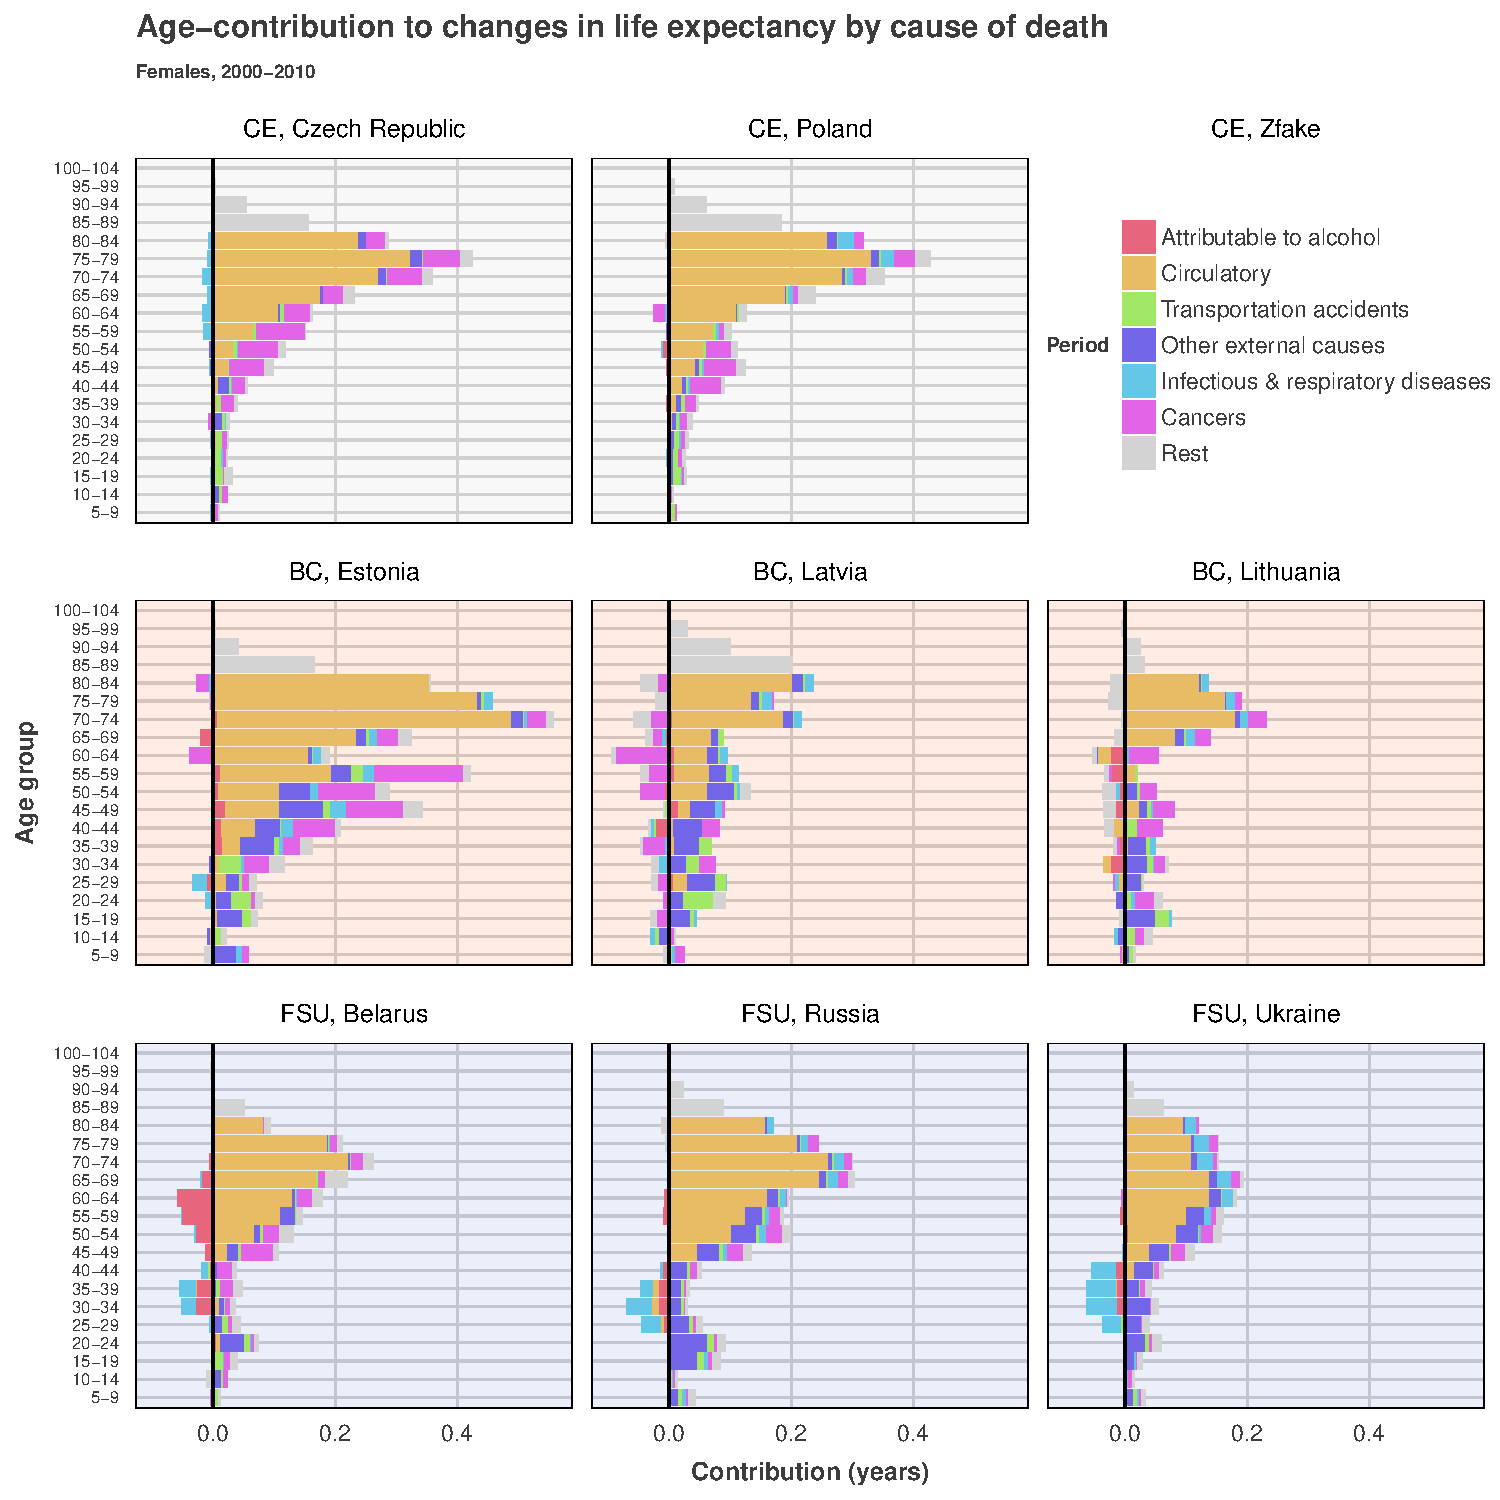
\includegraphics[scale=.5]{Figures/Cause_e0_decomp_Females_2.pdf}
\end{center}
Source: own calculations based on \citet{HMD} data. Note: data for Slovenia begins in 1983.
\end{figure}

\newpage
\section*{Sensitivity analysis without infant mortality and doubling infant mortality}

\subsection*{Conditional on surviving to age 5}
Figure 14 below shows life expectancy at age 5 versus life expectancy at birth for the Eastern European countries selected in our study. Although the levels differ, major trends are like the ones we show in the paper. For instance, Russia, Latvia and Estonia also show the lower values of life expectancy at age 5, and Slovenia and Czech Republic are the frontrunners in the region after 1990 for males, even without accounting for mortality below age 5.

Similarly, Figure 15 shows life disparity or lifespan variation conditional on surviving to age 5 and at birth. As in the previous figure, the trends are similar to lifespan variation over the full age span. Figure 16 shows the association between changes in life expectancy and lifespan variation conditional on surviving to age 5 and. The results do not change substantively compared to those including mortality under age 5.

We further performed the age-specific decomposition of lifespan variation conditional on surviving to age 5 following the same methodology that we used in the paper. Results are shown in Figure 17 below. The results are very close as if we decompose lifespan variation from age 0 (Figure 4 in the paper). 


\begin{figure}[h!]
\caption{Life expectancy at age 5 and life expectancy at birth for males.}
\centering
\begin{center}
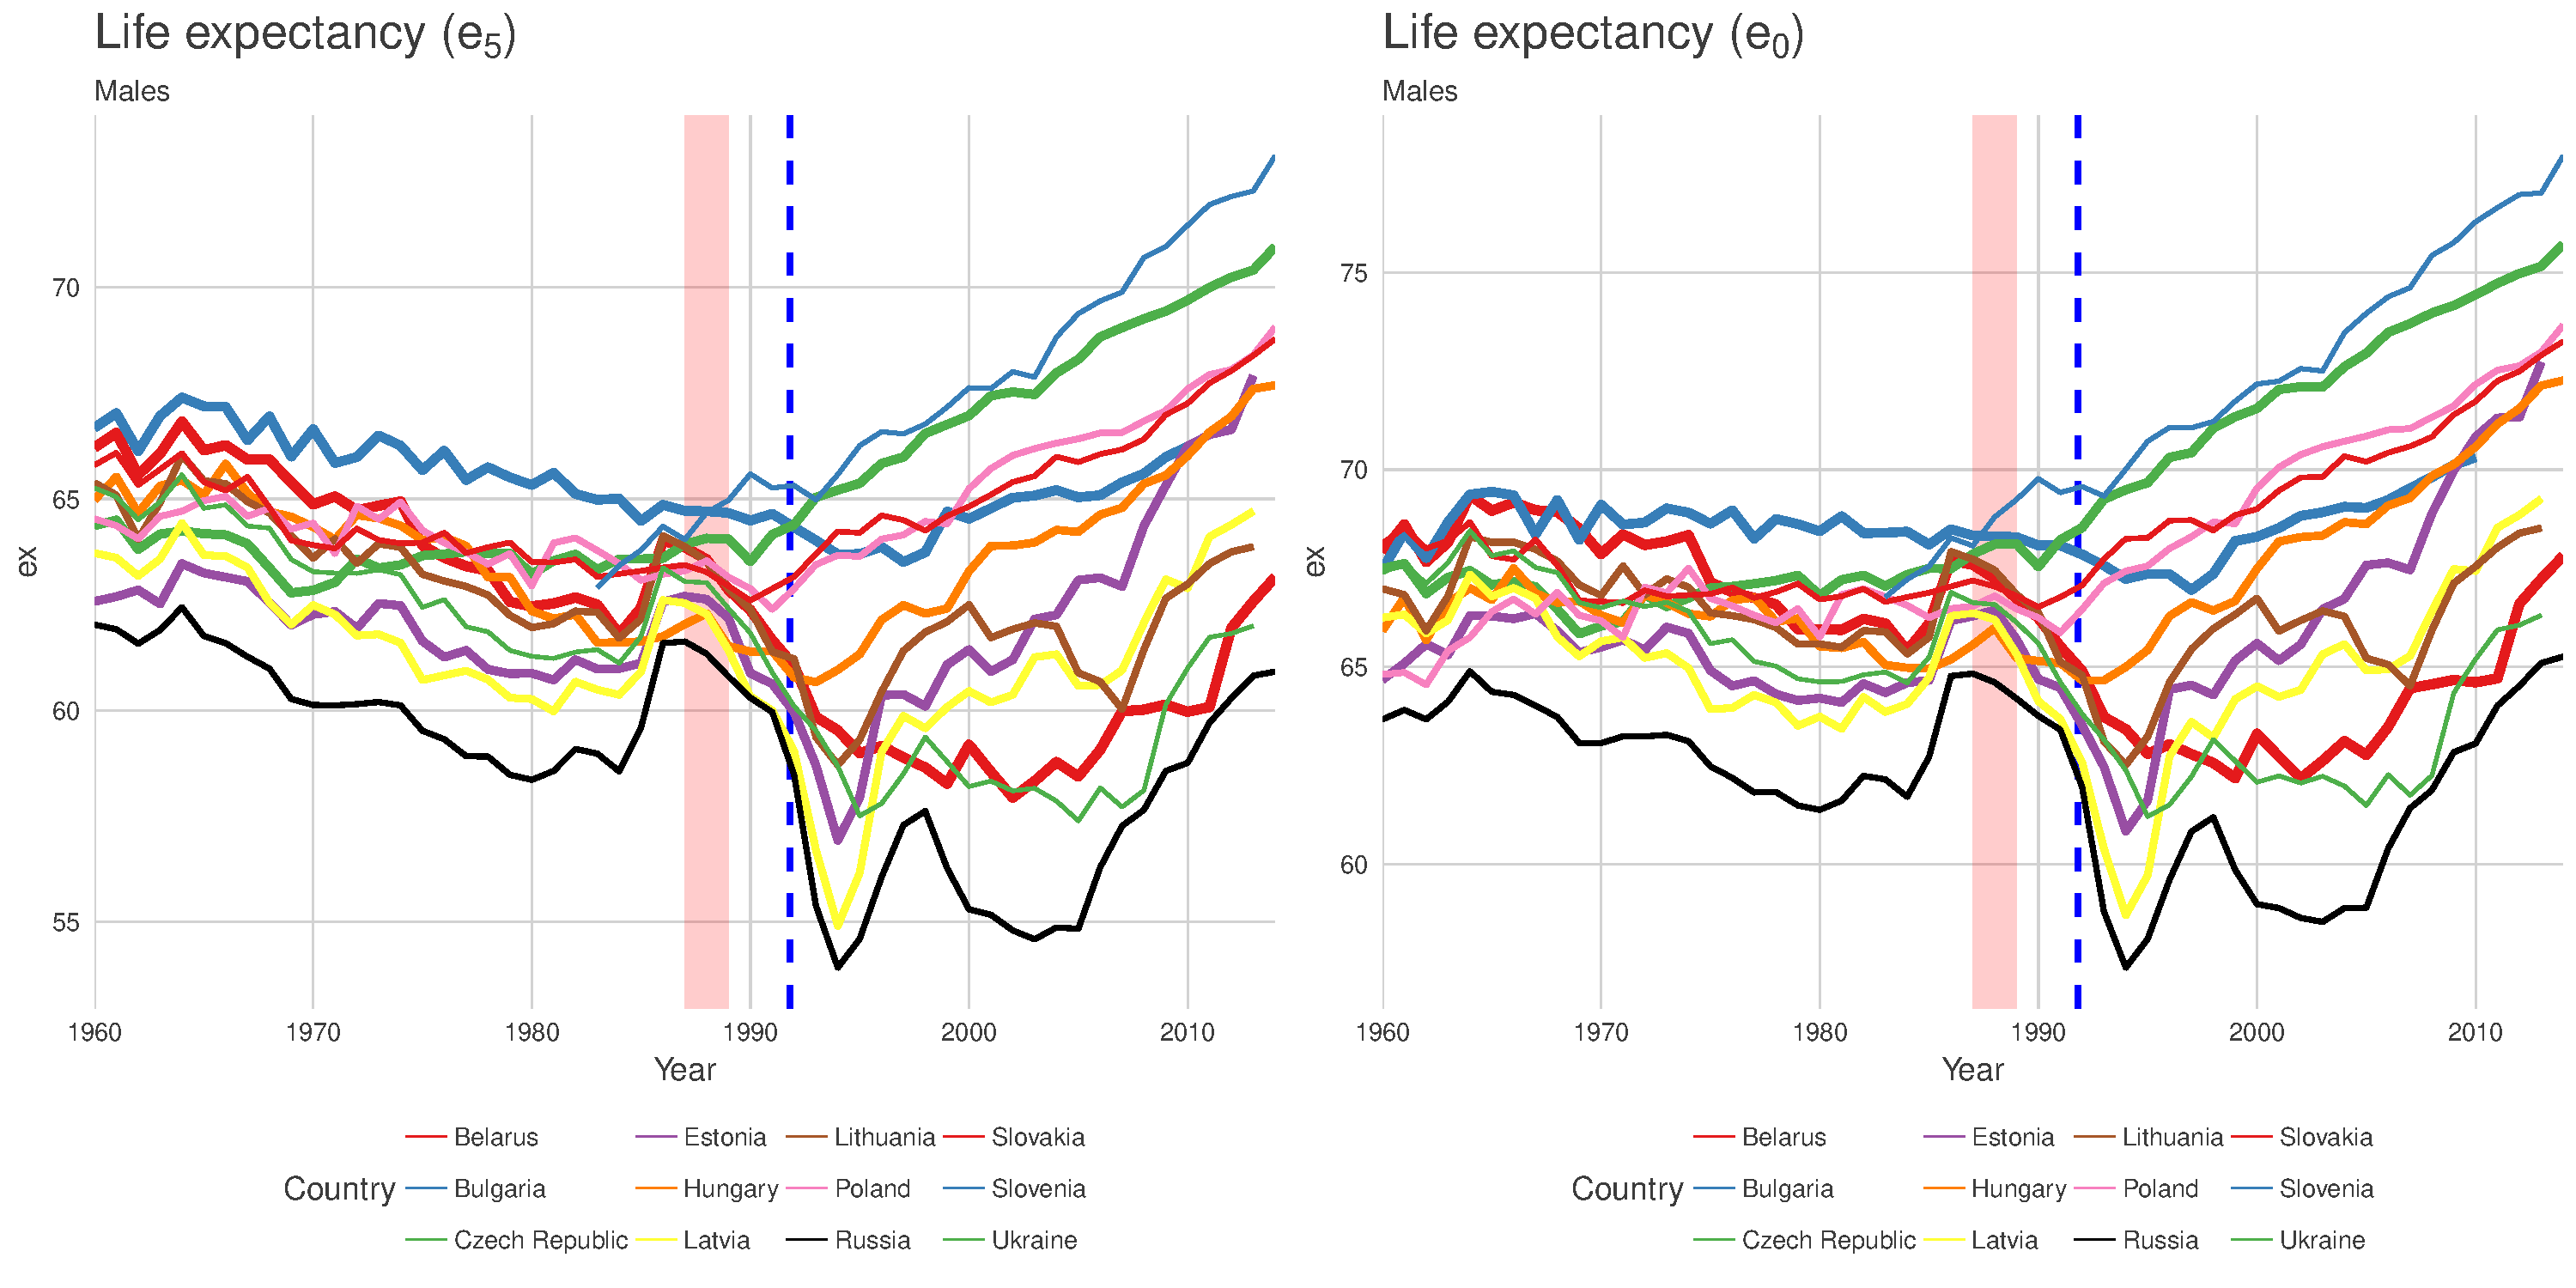
\includegraphics[scale=.35]{Figures/e5_0_males.pdf}
\end{center}
Source: own calculations based on \citet{HMD} data. Note: data for Slovenia begins in 1983.
\end{figure}

\newpage
\begin{figure}[h!]
\caption{Lifespan variation at age 5 and at birth for males.}
\centering
\begin{center}
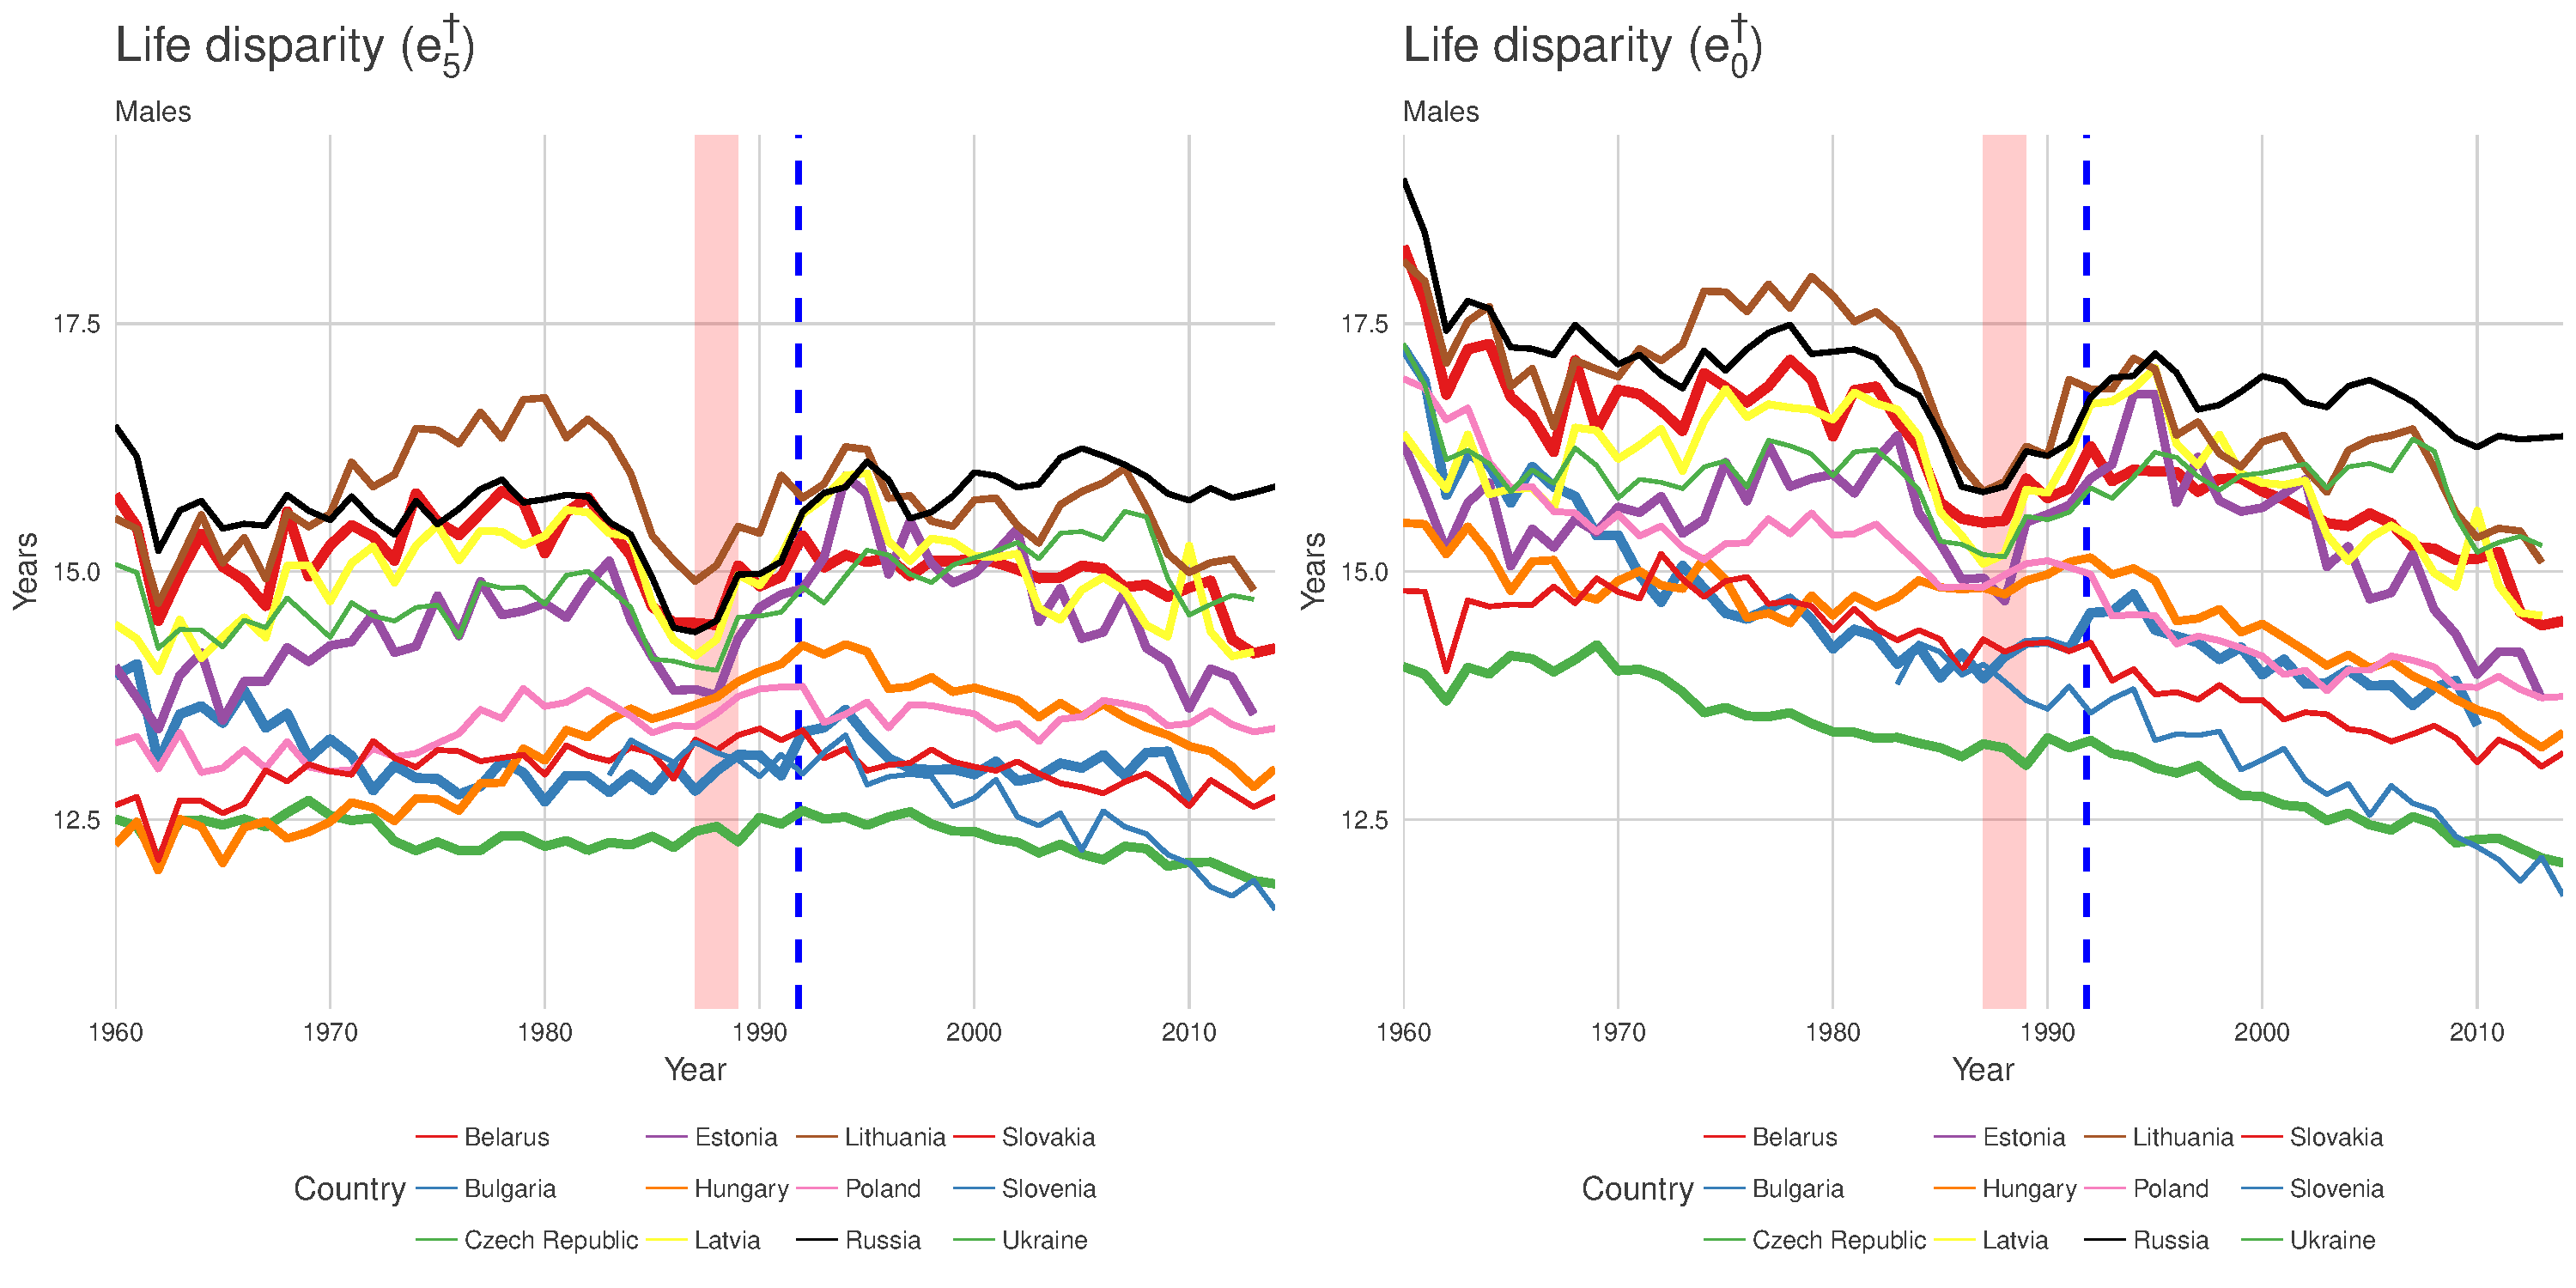
\includegraphics[scale=.35]{Figures/ed5_males-females.pdf}
\end{center}
Source: own calculations based on \citet{HMD} data. Note: data for Slovenia begins in 1983.
\end{figure}


\newpage
\begin{figure}[h!]
\caption{Association between changes in life expectancy at age 5 and lifespan variation conditional on surviving to age 5.}
\centering
\begin{center}
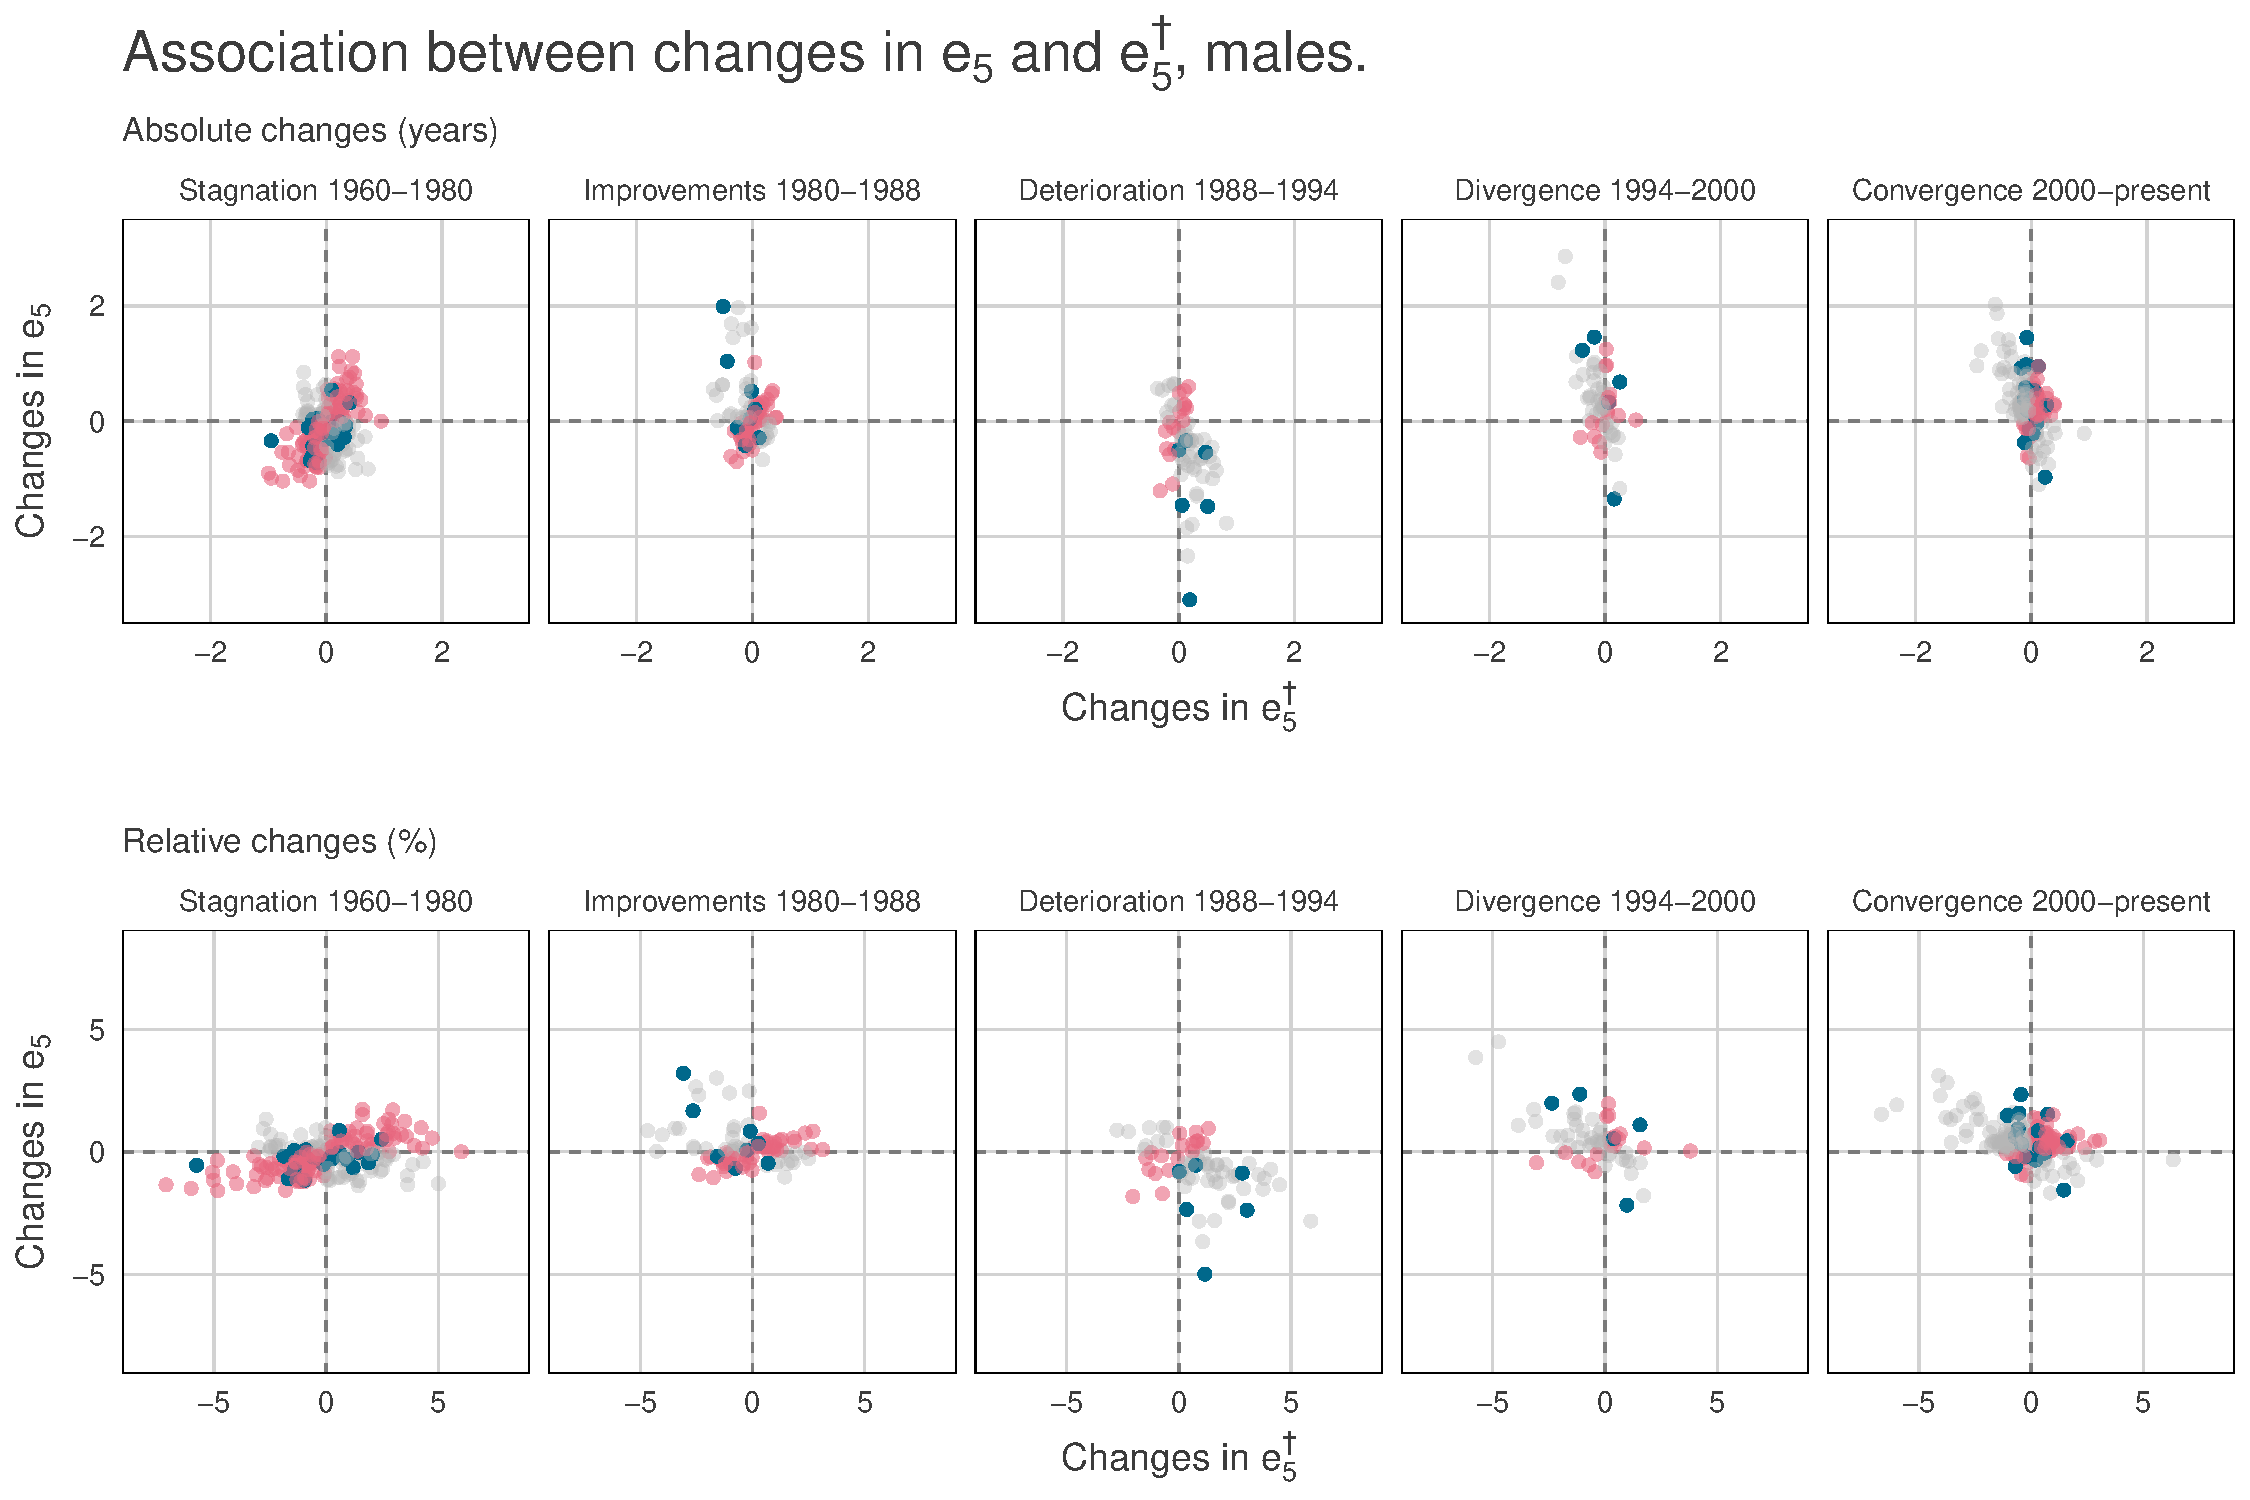
\includegraphics[scale=.45]{Figures/Changes_age5.pdf}
\end{center}
Source: own calculations based on \citet{HMD} data. Note: data for Slovenia begins in 1983.
\end{figure}

\newpage
\begin{figure}[h!]
\caption{Age specific decomposition for life expectancy and lifespan variation at age 5}
\centering
\begin{center}
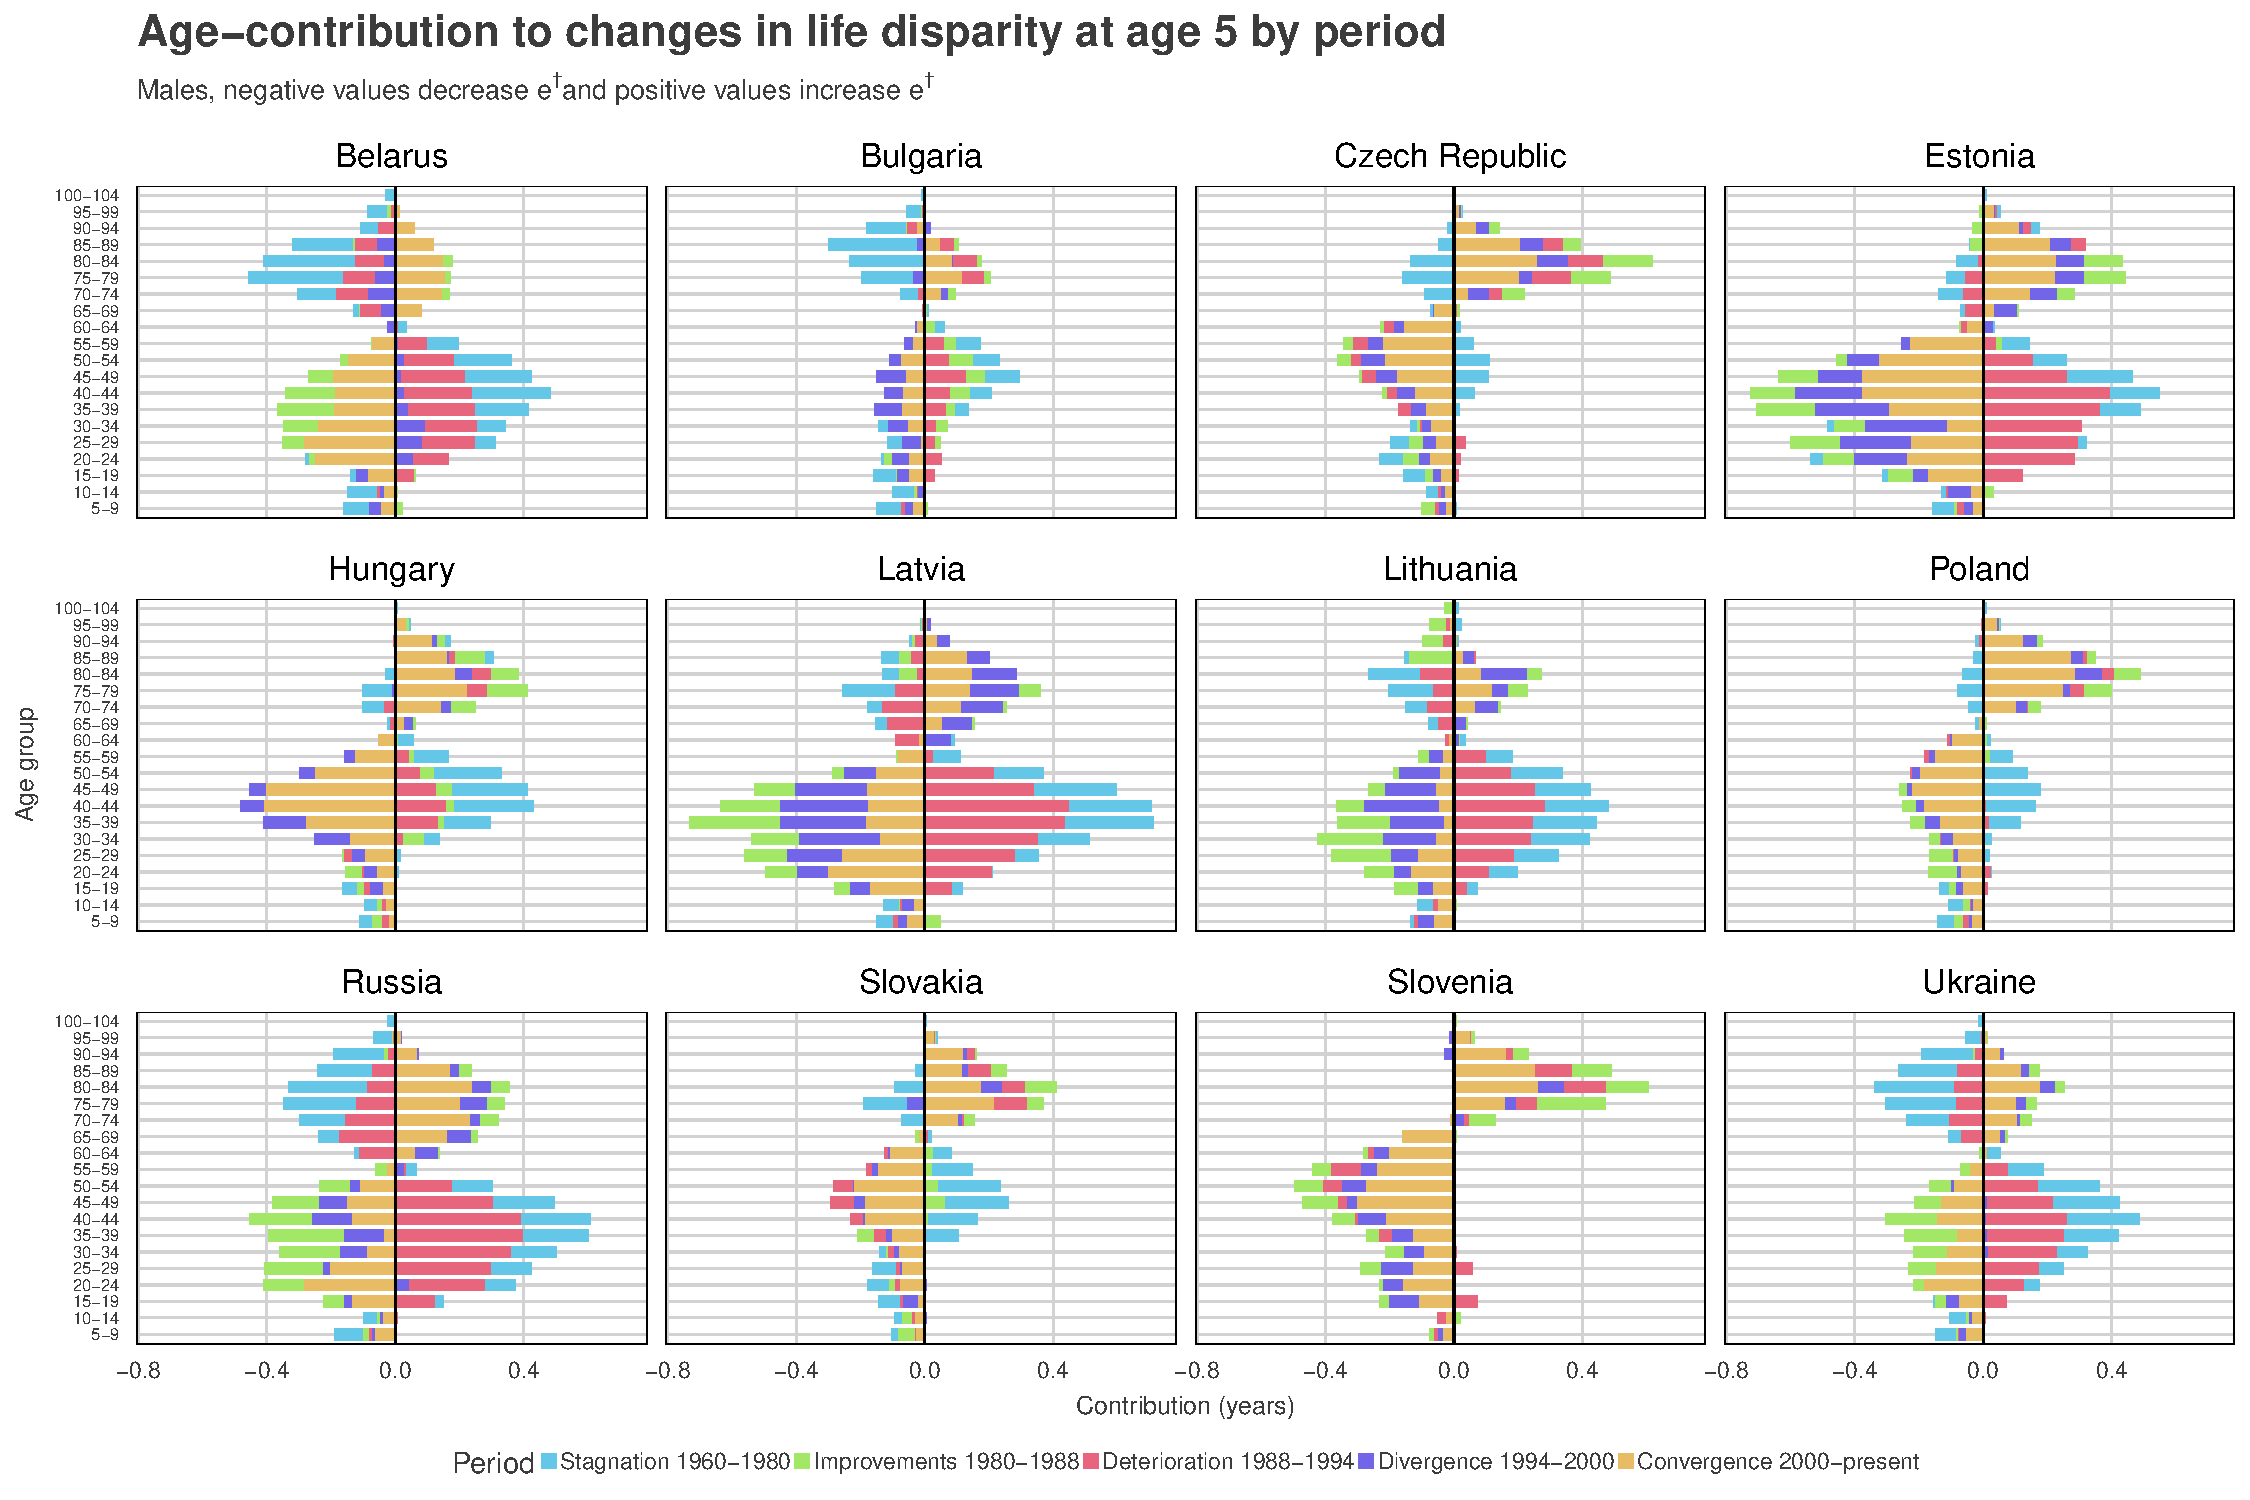
\includegraphics[scale=.45]{Figures/Decomp_ed_males_5.pdf}
\end{center}
Source: own calculations based on \citet{HMD} data. Note: data for Slovenia begins in 1983.
\end{figure}


\subsection*{Doubling infant mortality}
 To see the robustness check for different infant mortality scenarios follow \url{https://demographs.shinyapps.io/CEE_App/}
\newpage
\section*{Sensitivity analysis with the Gini coefficient}

\begin{figure}[h!]
\caption{Trends in life expectancy and Gini coefficient by sex for Eastern European countries}
\centering
\begin{center}
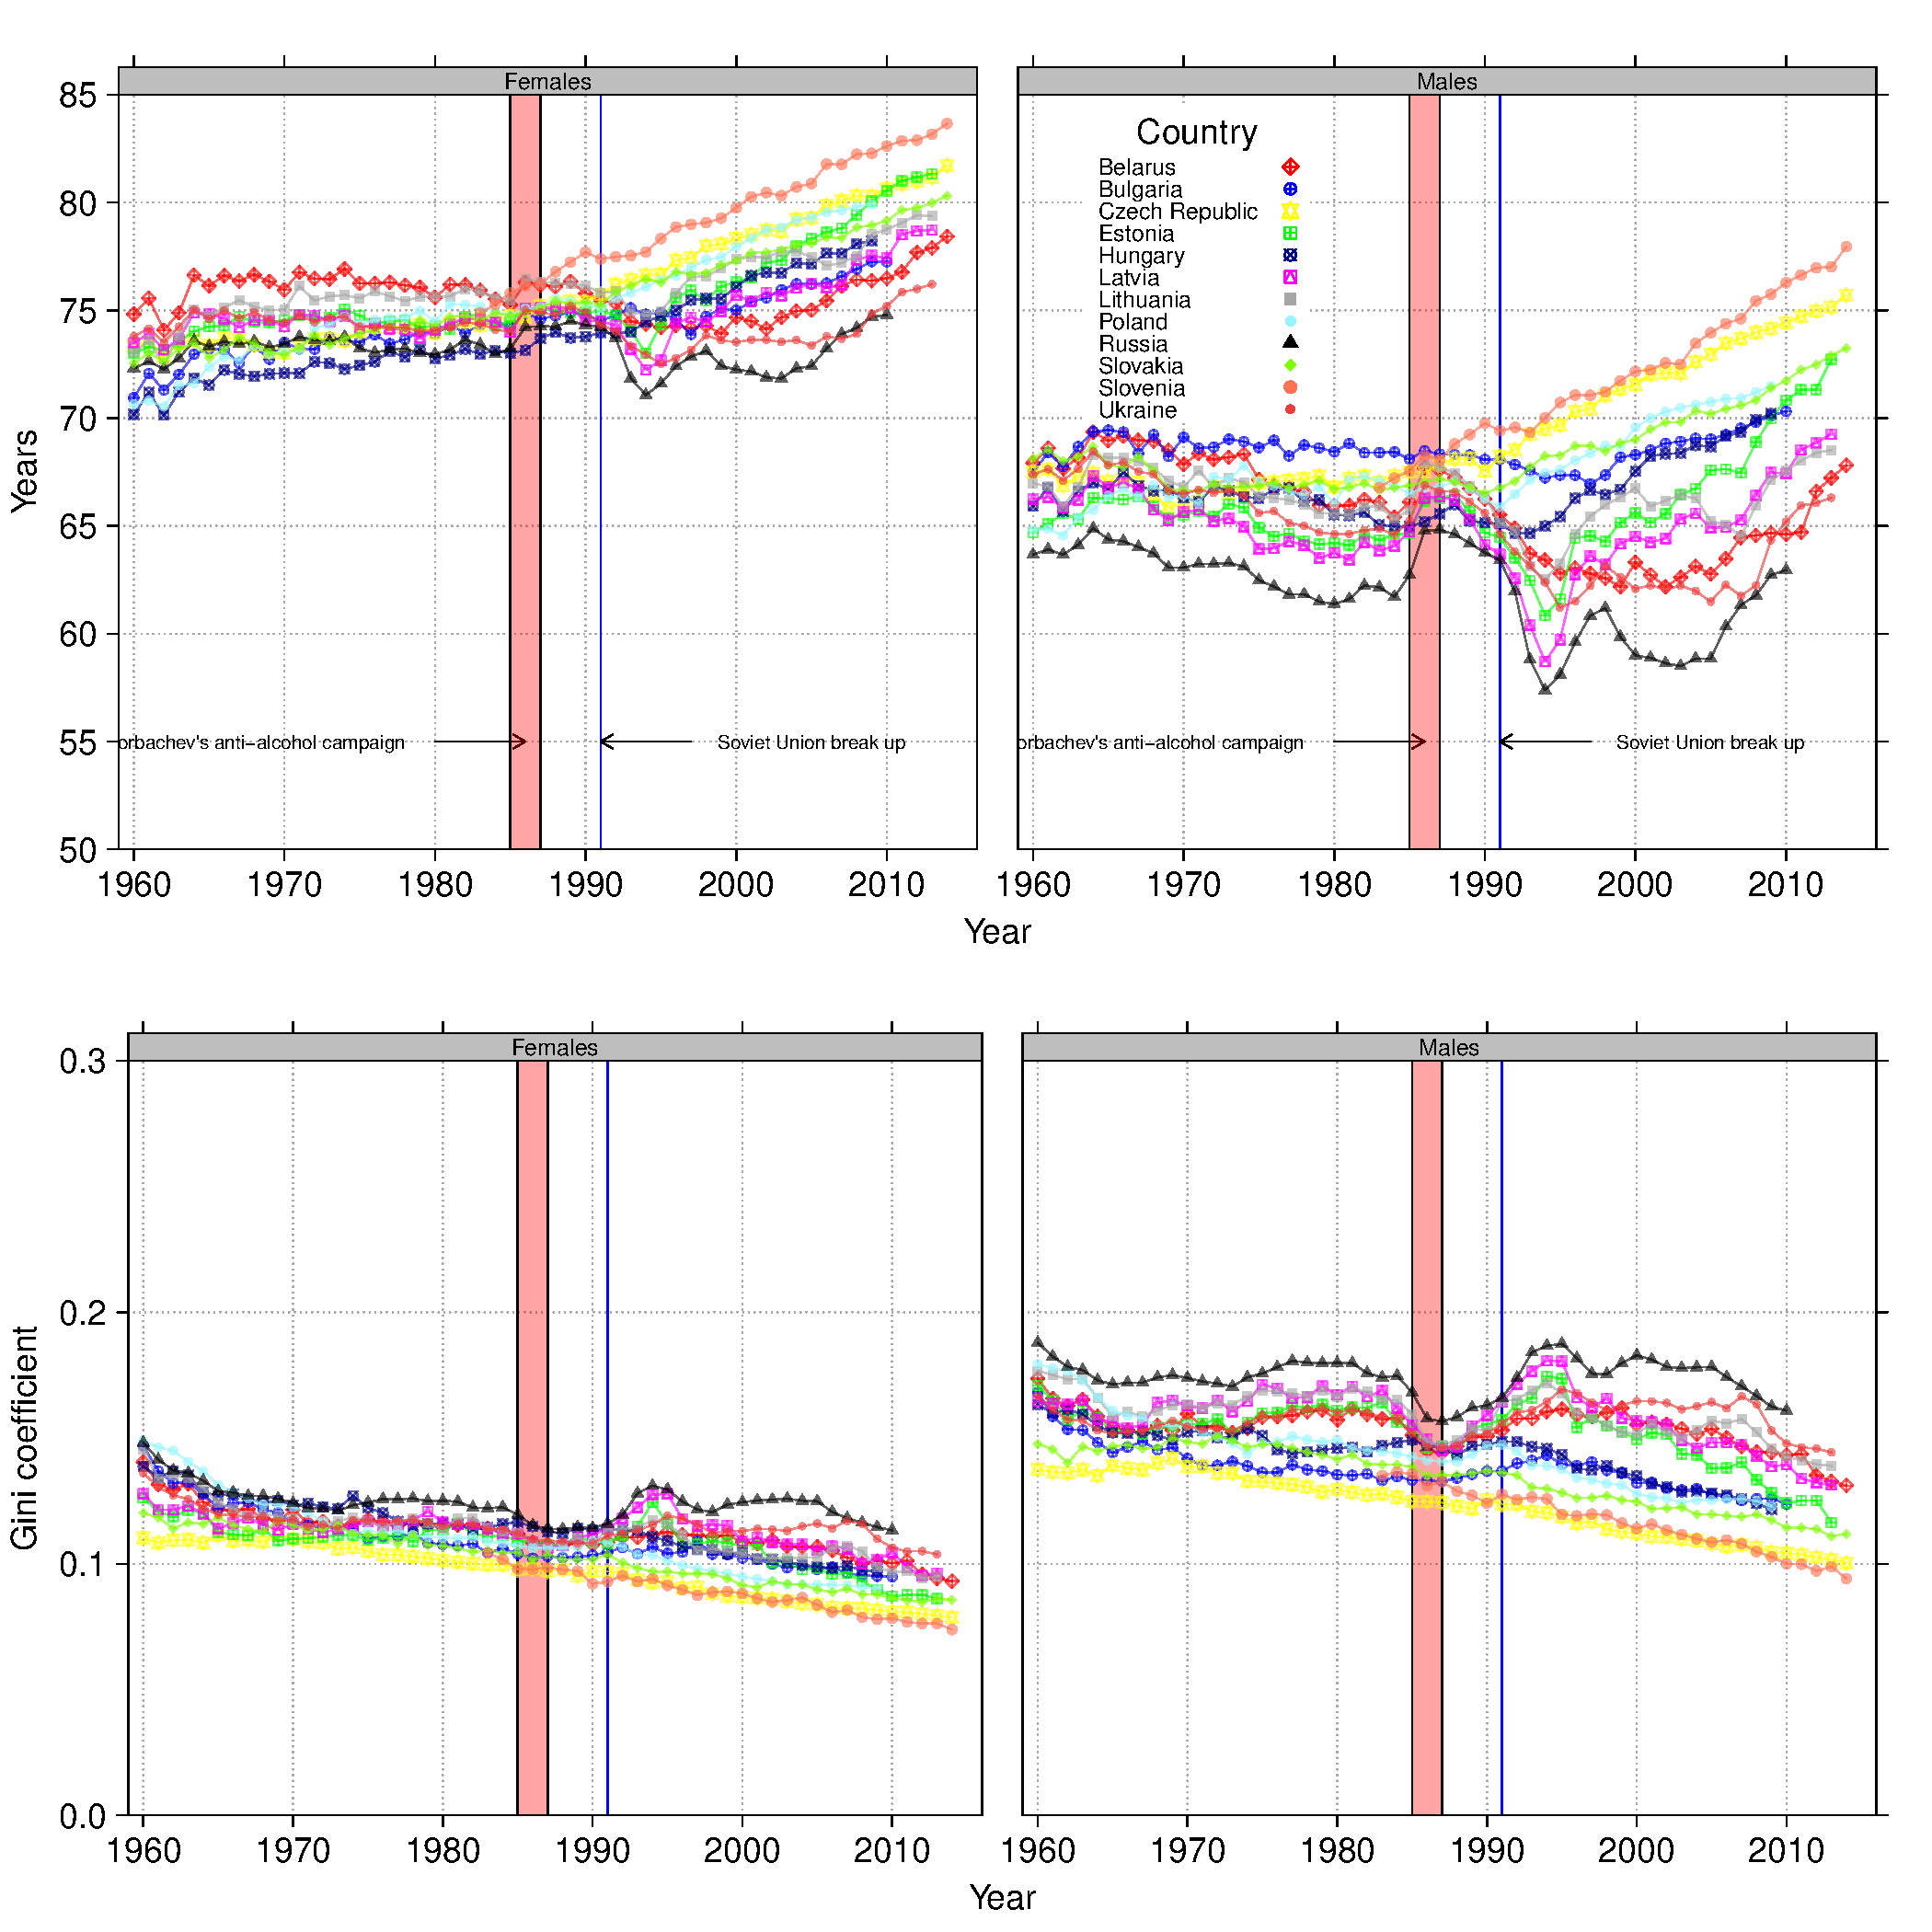
\includegraphics[scale=.4]{Figures/F1_SS}
\end{center}
\end{figure}

\newpage

\begin{figure}[h!]
\caption{Absolute changes in life expectancy and Gini coefficient by sex for Eastern European countries}
\centering
\begin{center}
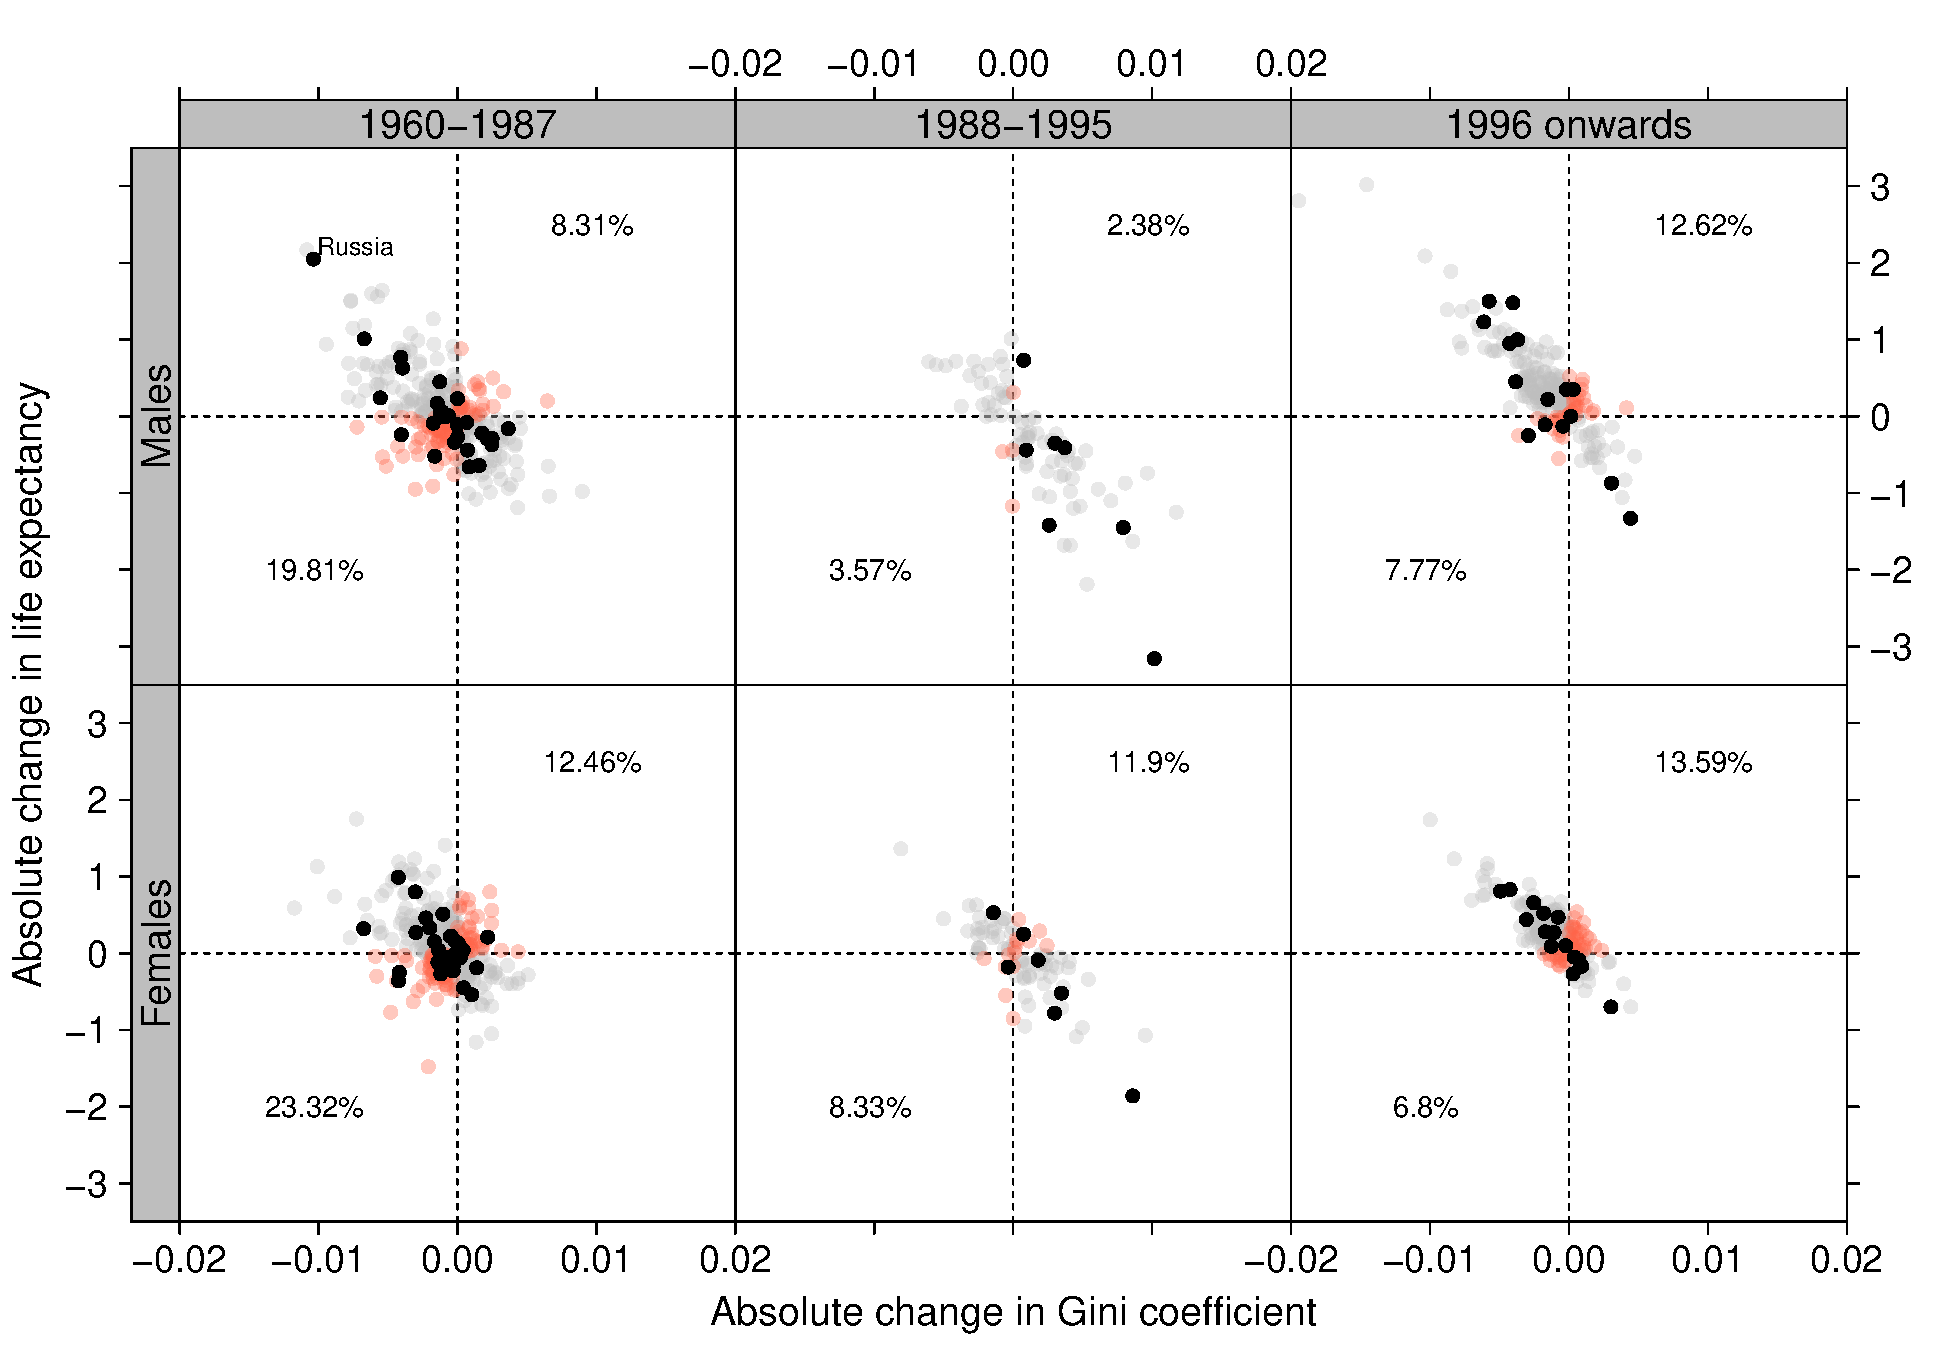
\includegraphics[scale=.4]{Figures/F2_SS}
\end{center}
\end{figure}

\newpage

\begin{figure}[h!]
\caption{Relative changes in life expectancy and Gini coefficient by sex for Eastern European countries}
\centering
\begin{center}
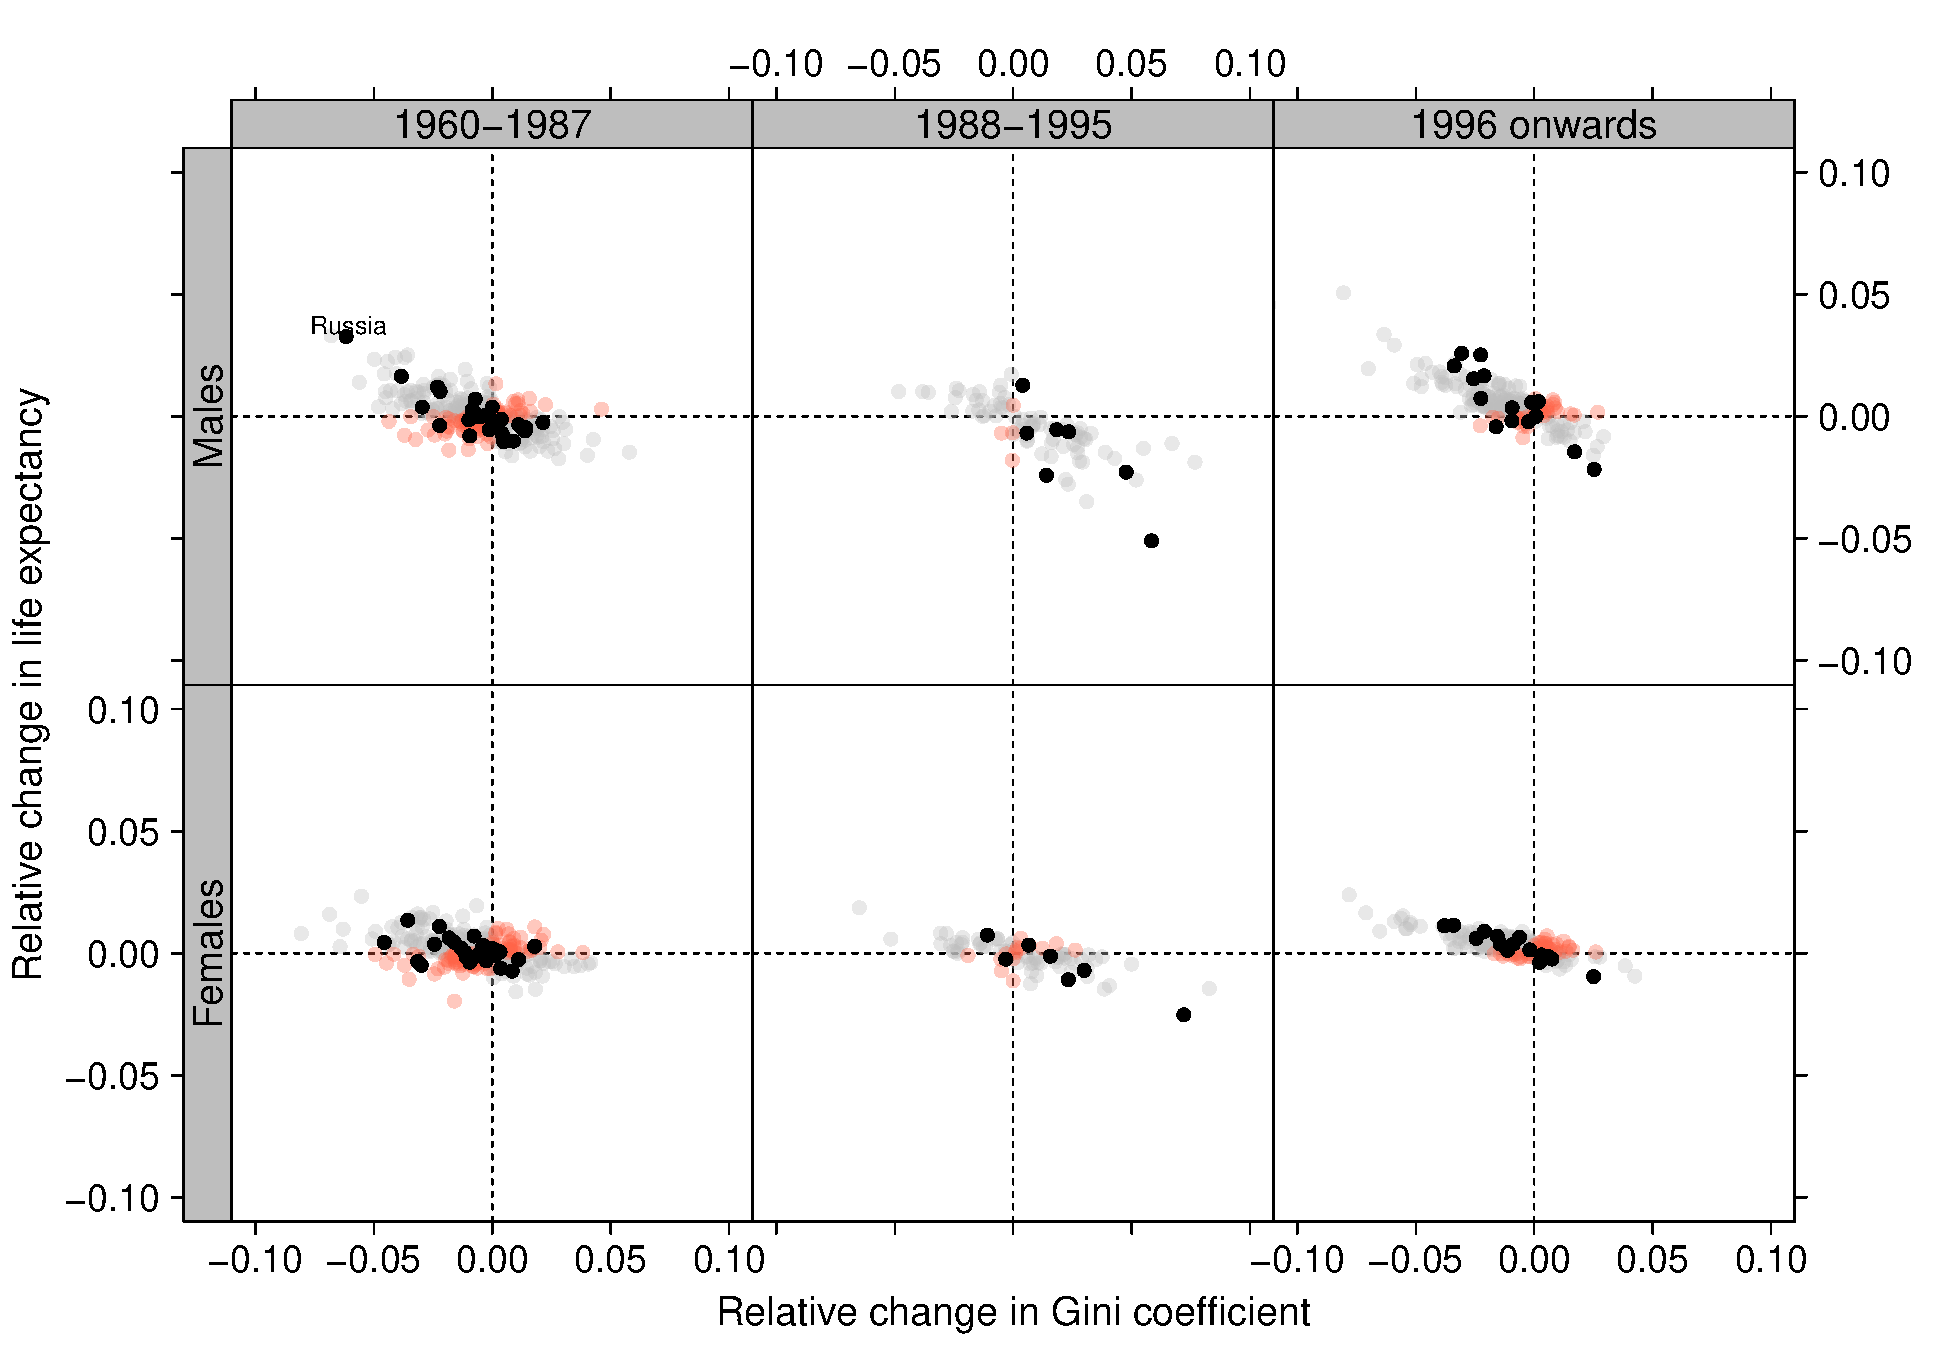
\includegraphics[scale=.4]{Figures/F3_SS}
\end{center}
\end{figure}

\newpage

\begin{figure}[h!]
\caption{Contributions to changes in Gini coefficient by period}
\centering
\begin{center}
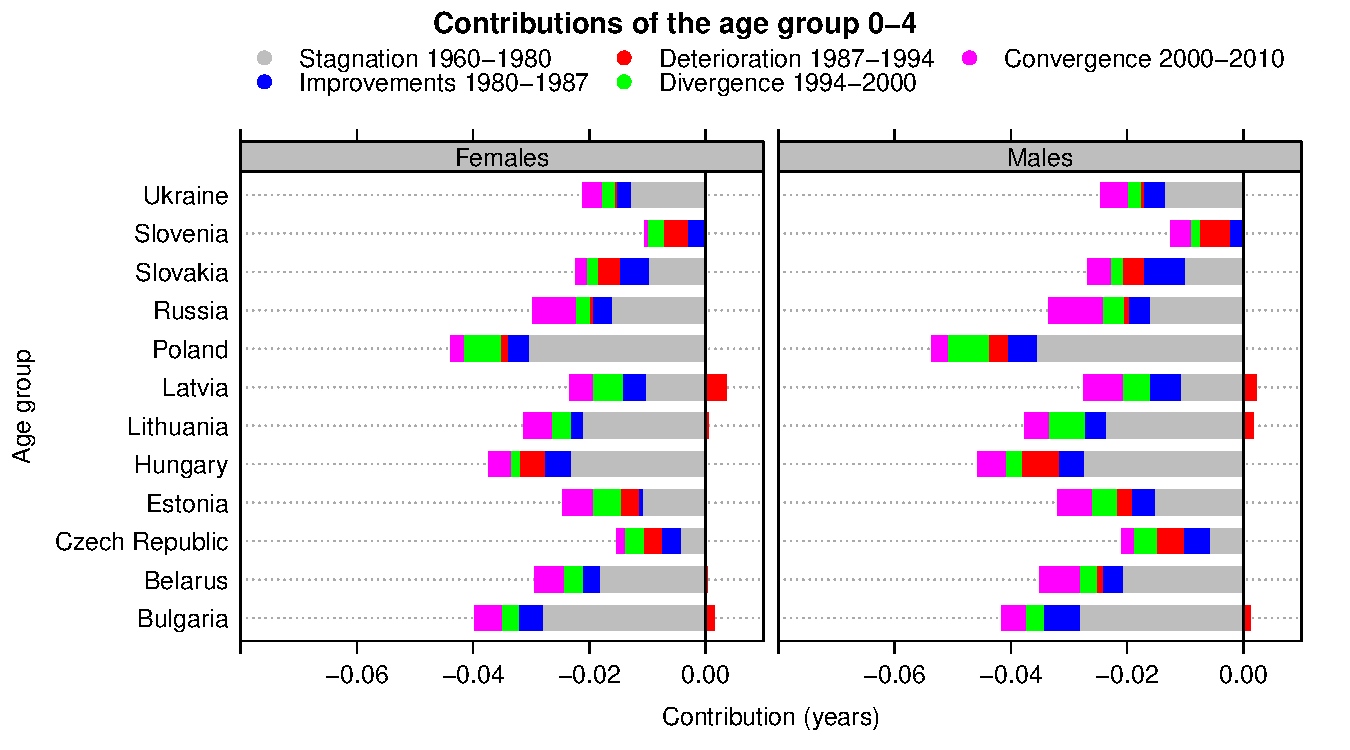
\includegraphics[scale=.6]{Figures/F6_SS_MalesInfant_Periods}
\end{center}
\end{figure}

\newpage

\begin{figure}[h!]
\caption{Contributions to changes in Gini coefficient by period, Males.}
\centering
\begin{center}
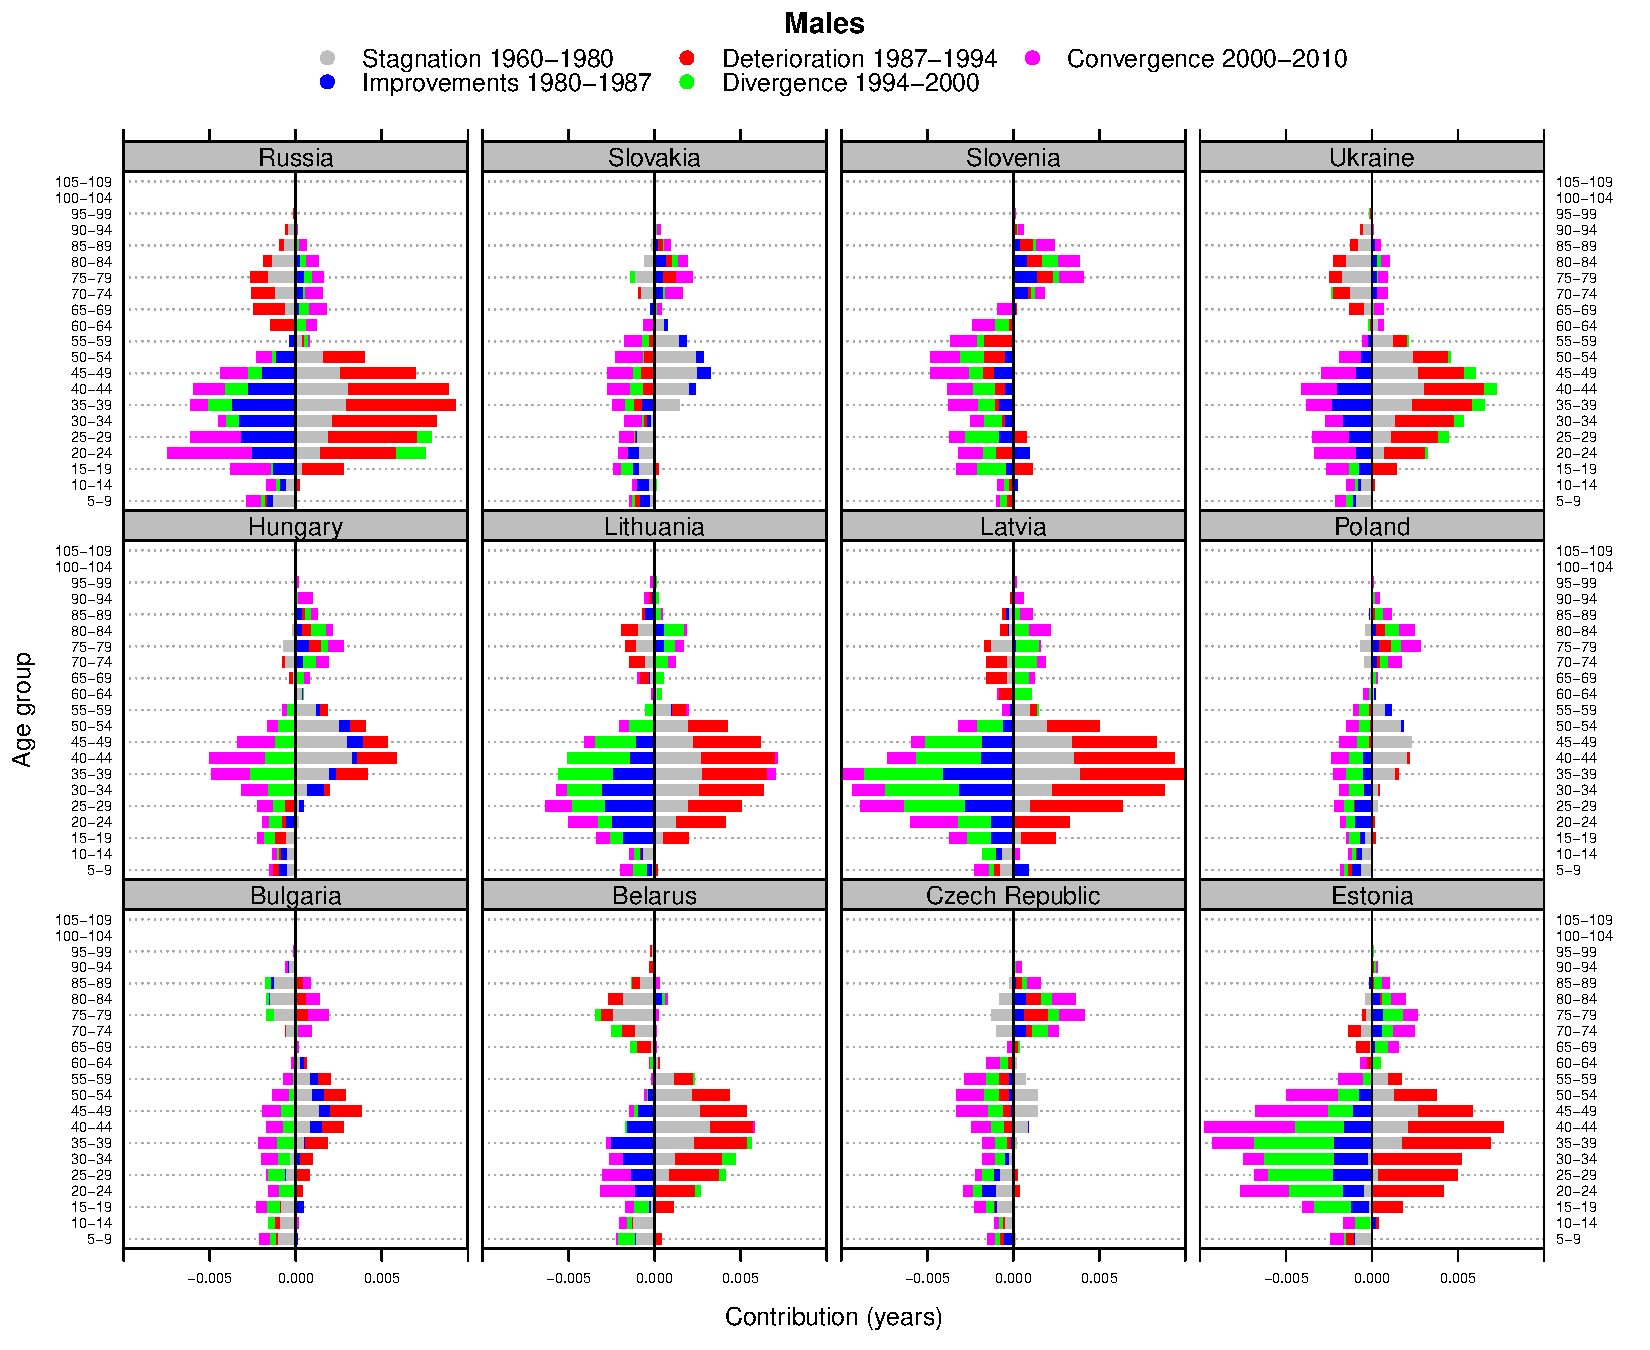
\includegraphics[scale=.54]{Figures/F4_SS_MalesDecomp_Periods}
\end{center}

\end{figure}



\newpage

 \bibliography{Aburto}


%}
%\bibliographystyle{plainnat}


\end{document}
